\documentclass[sigconf]{acmart}
 % Do not change for WSDM'20

\settopmatter{printacmref=true}
  % mandatory for WSDM'20

\fancyhead{}
  % do not delete this code.

\usepackage{balance}
  % for creating a balanced last page (usually last page with references)

% defining the \BibTeX command - from Oren Patashnik's original BibTeX documentation.
\def\BibTeX{{\rm B\kern-.05em{\sc i\kern-.025em b}\kern-.08emT\kern-.1667em\lower.7ex\hbox{E}\kern-.125emX}}
    
% Rights management information. 
% This information is sent to you when you complete the rights form.
% These commands have SAMPLE values in them; it is your responsibility as an author to replace
% the commands and values with those provided to you when you complete the rights form.
%
% These commands are for a PROCEEDINGS abstract or paper.

\usepackage{amsmath}
%\allowdisplaybreaks
\usepackage{amssymb}
%\usepackage{citehack}
%\usepackage{latexsym}
\usepackage{bm}
\usepackage{nicefrac}
\usepackage{booktabs}
\usepackage{array}
\usepackage{multirow}
\usepackage{threeparttable}
\usepackage{makecell}
\usepackage[procnumbered,ruled,vlined,linesnumbered]{algorithm2e}
\usepackage{siunitx}
\usepackage{stfloats}
\usepackage{graphicx}

\newcommand{\mR}{\ensuremath{\mathbf{R}}}
\newcommand{\Ncal}{\ensuremath{\mathcal{N}}}
\newcommand{\tr}[1]{\textrm{Tr} \left( #1 \right) }
\newcommand{\Cen}{\ensuremath{\mathcal{C}}}
%\newcommand{\b}[1]{\ensuremath{\mathbm{b}_{#1}}}
\newcommand{\UM}[1]{\ensuremath{\mathbf{I}_{#1}}}
\newcommand{\AO}[1]{\ensuremath{\mathbf{1}_{#1}}}
\newcommand{\dif}{\ensuremath{\mathrm{d}}}
\newcommand{\dv}[2]{\ensuremath{\frac{\mathrm{d} #1}{\mathrm{d} #2}}}
\newcommand{\pdv}[2]{\ensuremath{\frac{\partial #1}{\partial #2}}}

%\newcommand{\Kr}{\ensuremath{{K_f}}}

\newcommand{\yye}[1]{{\color{blue} #1}}
\newcommand{\ans}[1]{{\color{blue} #1}}

\newtheorem{problem}{Problem}
\newtheorem{theorem}{Theorem}[section]
\newtheorem{corollary}[theorem]{Corollary}
\newtheorem{lemma}[theorem]{Lemma}
\newtheorem{observation}[theorem]{Observation}
\newtheorem{proposition}[theorem]{Proposition}
\newtheorem{claim}[theorem]{Claim}
\newtheorem{fact}[theorem]{Fact}
\newtheorem{assumption}[theorem]{Assumption}
%\newtheorem{warning}[theorem]{Warning}
\def\proof{{\bf Proof.}\hskip 0.3truecm}
\def\endproof{\quad $\Box$}

\newtheorem{definition}[theorem]{Definition}
\newtheorem{remark}[theorem]{Remark}

\newenvironment{fminipage}%
{\begin{Sbox}\begin{minipage}}%
		{\end{minipage}\end{Sbox}\fbox{\TheSbox}}

\newenvironment{algbox}[0]{\vskip 0.2in
	\noindent
	\begin{fminipage}{6.3in}
	}{
	\end{fminipage}
	\vskip 0.2in
}

\def\pleq{\preccurlyeq}
\def\pgeq{\succcurlyeq}
\def\pge{\succ}
\def\ple{\prec}

\def\Approx#1{\approx_{#1}}

\newcommand{\E}{\mbox{{\bf E}}}

\def\defeq{\stackrel{\mathrm{def}}{=}}
\def\setof#1{\left\{#1  \right\}}
\def\sizeof#1{\left|#1  \right|}

\def\eps{\epsilon}

\def\abs#1{\left|#1  \right|}

\def\trace#1{\mathrm{Tr} \left(#1 \right)}
\def\norm#1{\left\| #1 \right\|}
\def\smallnorm#1{\| #1 \|}


\def\calC{\mathcal{C}}
\def\calE{\mathcal{E}}
\def\calG{\mathcal{G}}
\def\calL{\mathcal{L}}
\def\calS{\mathcal{S}}


\newcommand\Ppsi{\boldsymbol{\mathit{\Psi}}}
\newcommand\PPsi{\boldsymbol{\mathit{\Psi}}}
\newcommand\ppsi{\boldsymbol{\mathit{\psi}}}
\newcommand\pphi{\boldsymbol{\mathit{\phi}}}
\newcommand\Llambda{\boldsymbol{\mathit{\Lambda}}}
\newcommand\PPi{\boldsymbol{\Pi}}

\newcommand\ppi{\boldsymbol{\pi}}
\newcommand\cchi{\boldsymbol{\chi}}
\newcommand\aalpha{\boldsymbol{\alpha}}
\newcommand\bbeta{\boldsymbol{\beta}}
\newcommand\ggamma{\boldsymbol{\gamma}}
\newcommand\ddelta{\boldsymbol{\delta}}

\newcommand\er{R_{eff}}


\def\aa{\pmb{\mathit{a}}}
\newcommand\bb{\boldsymbol{\mathit{b}}}
\newcommand\cc{\boldsymbol{\mathit{c}}}
\newcommand\dd{\boldsymbol{\mathit{d}}}
\newcommand\ee{\boldsymbol{\mathit{e}}}
\newcommand\ff{\boldsymbol{\mathit{f}}}
\renewcommand\gg{\boldsymbol{\mathit{g}}}
\newcommand\ii{\boldsymbol{\mathit{i}}}
\newcommand\jj{\boldsymbol{\mathit{j}}}
\newcommand\kk{\boldsymbol{\mathit{k}}}
\renewcommand\ll{\boldsymbol{\mathit{l}}}
\newcommand\pp{\boldsymbol{\mathit{p}}}
\newcommand\qq{\boldsymbol{\mathit{q}}}
\newcommand\bs{\boldsymbol{\mathit{s}}}
\newcommand\nn{\boldsymbol{\mathit{n}}}
\newcommand\rr{\boldsymbol{\mathit{r}}}
\renewcommand\ss{\boldsymbol{\mathit{s}}}
\def\tt{\boldsymbol{\mathit{t}}}
\newcommand\uu{\boldsymbol{\mathit{u}}}
\renewcommand\vv{\boldsymbol{\mathit{v}}}
\newcommand\ww{\boldsymbol{\mathit{w}}}
\newcommand\yy{\boldsymbol{\mathit{y}}}
\newcommand\zz{\boldsymbol{\mathit{z}}}
\newcommand\xx{\boldsymbol{\mathit{x}}}
\newcommand\xxbar{\overline{\boldsymbol{\mathit{x}}}}

\renewcommand\AA{\boldsymbol{\mathit{A}}}
\newcommand\BB{\boldsymbol{\mathit{B}}}
\newcommand\CC{\boldsymbol{\mathit{C}}}
\newcommand\DD{\boldsymbol{\mathit{D}}}
\newcommand\EE{\boldsymbol{\mathit{E}}}
\newcommand\GG{\boldsymbol{\mathit{G}}}
\newcommand\II{\boldsymbol{\mathit{I}}}
\newcommand\JJ{\boldsymbol{\mathit{J}}}
\newcommand\KK{\boldsymbol{\mathit{K}}}
\newcommand\NN{\boldsymbol{\mathit{N}}}
\newcommand\MM{\boldsymbol{\mathit{M}}}
\newcommand\LL{\boldsymbol{\mathit{L}}}
\newcommand\PP{\boldsymbol{\mathit{P}}}
\newcommand\QQ{\boldsymbol{\mathit{Q}}}
\newcommand\RR{\boldsymbol{\mathit{R}}}
\renewcommand\SS{\boldsymbol{\mathit{S}}}
\newcommand\UU{\boldsymbol{\mathit{U}}}
\newcommand\WW{\boldsymbol{\mathit{W}}}
\newcommand\VV{\boldsymbol{\mathit{V}}}
\newcommand\XX{\boldsymbol{\mathit{X}}}
\newcommand\YY{\boldsymbol{\mathit{Y}}}
\newcommand\ZR{\boldsymbol{\mathit{0}}}


\newcommand\MMtil{\boldsymbol{\mathit{\tilde{M}}}}
\newcommand\ZZtil{\boldsymbol{\mathit{\tilde{Z}}}}
\newcommand\AAtilde{\boldsymbol{\mathit{\tilde{A}}}}
\newcommand\LLtil{\boldsymbol{\mathit{\tilde{L}}}}
\newcommand\MMtilde{\boldsymbol{\mathit{\tilde{M}}}}

\newcommand\AAn{\boldsymbol{\mathcal{A}}}
\newcommand\ZZ{\boldsymbol{\mathit{Z}}}

\newcommand\AAhat{\boldsymbol{\widehat{\mathit{A}}}}
\newcommand\AAapprox{\boldsymbol{\widetilde{\mathit{A}}}}
\newcommand\DDhat{\boldsymbol{\widehat{\mathit{D}}}}
\newcommand\DDapprox{\boldsymbol{\widetilde{\mathit{D}}}}
\newcommand\LLhat{\boldsymbol{\widehat{\mathit{L}}}}
\newcommand\LLapprox{\boldsymbol{\widetilde{\mathit{L}}}}
\newcommand\MMhat{\boldsymbol{\widehat{\mathit{M}}}}
\newcommand\MMapprox{\boldsymbol{\widetilde{\mathit{M}}}}
\newcommand\ZZhat{\boldsymbol{\widehat{\mathit{Z}}}}

\newcommand\AAtil{\boldsymbol{\widetilde{\mathit{A}}}}
\newcommand\DDtil{\boldsymbol{\widetilde{\mathit{D}}}}


\newcommand\bbtil{\boldsymbol{\tilde{\mathit{b}}}}
\newcommand\xxtil{\boldsymbol{\tilde{\mathit{x}}}}


\newcommand\Otil{\widetilde{O}}

\newcommand\Tcal{\mathcal{T}}

\newcommand\xhat{\boldsymbol{\hat{\mathit{x}}}}
\newcommand\uhat{{\hat{{u}}}}
\newcommand\vhat{{\hat{{v}}}}
\newcommand\what{{\hat{{w}}}}

\newcommand\Ghat{{\widehat{{G}}}}

\newcommand{\sym}[1]{\mathrm{sym} (#1)}
\newcommand{\bsk}{\backslash_{\theta}}

\newcommand{\one}{\mathbf{1}}
\newcommand{\diag}{\textsc{diag}}
\newcommand\LLs{\boldsymbol{\mathit{L}_s}}

\newcommand{\todo}[1]{{\bf \color{red} TODO: #1}}
\newcommand{\yhy}[1]{{\bf \color{green} Yuhao: #1}}
\newcommand{\lrs}[1]{{\bf \color{green} Liren: #1}}
\newcommand{\zzz}[1]{{\bf \color{green} Zhongzhi: #1}}

\newcommand{\expct}[2]{\ensuremath{\mathop{\text{\normalfont \textbf{E}}}_{#1}}\left[#2\right]}

\DeclareMathOperator*{\argmin}{arg\,min}
\DeclareMathOperator*{\argmax}{arg\,max}

\newcommand{\kh}[1]{\left(#1\right)}

% Algorithm2e
\DontPrintSemicolon
\SetKw{KwAnd}{and}
%\SetProcnameSty{textsc}
\SetFuncSty{textsc}
\SetKwInOut{Input}{Input\ \ \ \ }
\SetKwInOut{Output}{Output}


\usepackage{tabularx}
\usepackage{stfloats}


\copyrightyear{2020}
\acmYear{2020}
\setcopyright{acmcopyright}
\acmConference[WSDM '20]{The Thirteenth ACM International Conference on Web Search and Data Mining}{February 3--7, 2020}{Houston, TX, USA}
\acmBooktitle{The Thirteenth ACM International Conference on Web Search and Data Mining (WSDM '20), February 3--7, 2020, Houston, TX, USA}
\acmPrice{15.00}
\acmDOI{10.1145/3336191.3371777}
\acmISBN{978-1-4503-6822-3/20/02}



%%
%% The majority of ACM publications use numbered citations and
%% references.  The command \citestyle{authoryear} switches to the
%% "author year" style.
%%
%% If you are preparing content for an event
%% sponsored by ACM SIGGRAPH, you must use the "author year" style of
%% citations and references.
%% Uncommenting
%% the next command will enable that style.
%%\citestyle{acmauthoryear}

%%
%% end of the preamble, start of the body of the document source.
\begin{document}
\fancyhead{}
%%
%% The "title" command has an optional parameter,
%% allowing the author to define a "short title" to be used in page headers.
\title{Nearly Linear Time Algorithm for Mean Hitting Times of Random Walks on a Graph}
\titlenote{The authors are with the Shanghai Key Laboratory of Intelligent Information Processing, School of Computer Science, Fudan University, Shanghai, 200433, China.}

%%
%% The "author" command and its associated commands are used to define
%% the authors and their affiliations.
%% Of note is the shared affiliation of the first two authors, and the
%% "authornote" and "authornotemark" commands
%% used to denote shared contribution to the research.

\author{Zuobai Zhang}
\affiliation{%
	\institution{Fudan University}
	%\streetaddress{1 Th{\o}rv{\"a}ld Circle}
	\city{Shanghai}
	\country{China}}
\email{17300240035@fudan.edu.cn}

\author{Wanyue Xu}
\affiliation{%
	\institution{Fudan University}
	%\streetaddress{1 Th{\o}rv{\"a}ld Circle}
	\city{Shanghai}
	\country{China}}
\email{xuwy@fudan.edu.cn}

\author{Zhongzhi Zhang}
\authornote{Corresponding author.}
\affiliation{%
	\institution{Fudan University}
	%\streetaddress{1 Th{\o}rv{\"a}ld Circle}
	\city{Shanghai}
	\country{China}}
\email{zhangzz@fudan.edu.cn}

%
% By default, the full list of authors will be used in the page headers. Often, this list is too long, and will overlap
% other information printed in the page headers. This command allows the author to define a more concise list
% of authors' names for this purpose.
\renewcommand{\shortauthors}{Z. Zhang, W. Xu, and Z. Zhang.}

%%
%% The abstract is a short summary of the work to be presented in the
%% article.
\begin{abstract}
	For random walks on a graph, the mean hitting time $H_j$ from a vertex $i$ chosen from the stationary distribution to the target vertex $j$ can be used as a measure of importance for vertex  $j$, while the Kemeny constant $K$ is the mean hitting time from a vertex $i$ to a vertex $j$ selected randomly according to the stationary distribution. Both quantities have found a large variety of applications in different areas. However, their high computational complexity limits their applications, especially for large networks with millions of vertices. In this paper, we first establish a connection between the two quantities, representing $K$ in terms of $H_j$ for all vertices. We then express both quantities in terms of quadratic forms of the pseudoinverse for graph Laplacian, based on which we develop an efficient algorithm that provides an approximation of $H_j$ for all vertices and $K$ in nearly linear time with respect to  the edge number, with  high probability. Extensive experiment results on real-life and model networks validate both the efficiency and accuracy of the proposed algorithm.
\end{abstract}

%%
%% The code below is generated by the tool at http://dl.acm.org/ccs.cfm.
%% Please copy and paste the code instead of the example below.
%%
\begin{CCSXML}
	<ccs2012>
	<concept>
	<concept_id>10002951.10003227.10003351</concept_id>
	<concept_desc>Information systems~Data mining</concept_desc>
	<concept_significance>500</concept_significance>
	</concept>
	<concept>
	<concept_id>10003752.10003809.10003635</concept_id>
	<concept_desc>Theory of computation~Graph algorithms analysis</concept_desc>
	<concept_significance>500</concept_significance>
	</concept>
	<concept>
	<concept_id>10003752.10003809.10003636</concept_id>
	<concept_desc>Theory of computation~Approximation algorithms analysis</concept_desc>
	<concept_significance>500</concept_significance>
	</concept>
	</ccs2012>
\end{CCSXML}

\ccsdesc[500]{Information systems~Data mining}
\ccsdesc[500]{Theory of computation~Graph algorithms analysis}
\ccsdesc[500]{Theory of computation~Approximation algorithms analysis}

%%
%% Keywords. The author(s) should pick words that accurately describe
%% the work being presented. Separate the keywords with commas.
\keywords{Random walk; hitting time; Kemeny constant; spectral algorithm; complex network; node centrality}

%% A "teaser" image appears between the author and affiliation
%% information and the body of the document, and typically spans the
%% page.
%	\begin{teaserfigure}
%		\includegraphics[width=\textwidth]{sampleteaser}
%		\caption{Seattle Mariners at Spring Training, 2010.}
%		\Description{Enjoying the baseball game from the third-base
%			seats. Ichiro Suzuki preparing to bat.}
%		\label{fig:teaser}
%	\end{teaserfigure}

%%
%% This command processes the author and affiliation and title
%% information and builds the first part of the formatted document.
\maketitle



\section{Introduction}

As a powerful tool and method, random walks have found broad applications in various aspects. Frequently cited examples include image segmentation~\cite{Le06}, random algorithm design~\cite{SaDi12}, collaborative recommendation~\cite{FoPiReSa07}, community detection~\cite{LaDeBa14}, among others. A fundamental quantity related to random walks is hitting time~\cite{Lo93}, also called first-passage time~\cite{CoBeTeVoKl07}. For a random walk on a graph, the hitting time $H_{ij}$ from a vertex $i$ to another vertex $j$ is the expected time for the walker starting from $i$ to visit $j$ for the first time. Hitting time is related to many problems and has been successfully applied to diverse areas, such as Hanoi problem with random move~\cite{WuZhCh11}, query suggestion~\cite{MeZhCh08}, and clustering algorithm~\cite{ChLiTa08}.

Except for the intrinsic interest of hitting time itself and its direct applications, many other relevant quantities related to random walks are encoded in or expressed in terms of this crucial quantity, for example, absorbing random-walk centrality~\cite{MaMagi15} (or Markov centrality~\cite{WhSm03}) and Kemeny constant~\cite{Hu14}, both of which are a partial average of hitting times. As the name implies, the absorbing random-walk centrality is a measure for the importance of vertices on a graph. For a vertex $j$, its absorbing random-walk centrality $H_j$ is defined by $H_j=\sum_{i} \rho(i) H_{ij}$, where $\rho(\cdot)$ is the starting probability distribution over all vertices. Different from the shortest-path based centrality measures, random-walk based centrality metrics include the contributions from essentially all paths~\cite{Ne05}, and thus have a better discriminating power.

For random walks on a graph with $n$ vertices, the Kemeny constant $K$ is defined as the expected time for the walker starting from one vertex to second vertex selected randomly from the graph according to the stationary distribution $\ppi=(\pi_1, \pi_2, \cdots, \pi_n)^{\top}$ of the random walk, that is, $K=\sum_{j} \pi_j H_{ij}$. The Kemeny constant has also found a wealth of applications in different fields~\cite{Hu14}. It can be utilized to gauge the efficiency of user navigation through the World Wide Web (WWW)~\cite{LeLo02}. Moreover, the Kemeny constant is related to the mixing rate of an irreducible Markov chain~\cite{LePeWi09}, by regarding it as the expected time to mixing of the Markov chain~\cite{Hu06}. Recently, the Kemeny constant has been applied to measure the efficiency of robotic surveillance in network environments~\cite{PaAgBu15} and to characterize the noise robustness of a class of protocols for formation control~\cite{JaOl19}.


Despite the wide range of applications of the absorbing random-walk centrality and the Kemeny constant, it is a computational challenge to obtain their exact values. By definition, both the absorbing random-walk centrality and the Kemeny constant are a partial average of some hitting times. However, the exact value of hitting time between any pair of vertices in a graph involves all eigenvalues and eigenvectors of (normalized) Laplacian matrix associated with the graph~\cite{Lo93,LiZh13PRE}, the computation complexity of which is the cube of the vertex number. Thus, for large realistic networks with millions of vertices, we cannot obtain their absorbing random-walk centrality and the Kemeny constant by resorting this straightforward method for computing hitting time.  It is then of theoretical and practical interest to seek for alternative approximate approaches that scale to large networks.

In this paper, we propose a nearly linear time algorithm to address the computation issue for absorbing random-walk centrality  $H_j$ and Kemeny constant $K$ in large networks. We focus on a special absorbing random-walk centrality $H_j=\sum_{i} \rho(i) H_{ij}$, with the starting probability distribution $\rho(\cdot)$ being the stationary distribution $\ppi=(\pi_1, \pi_2, \cdots, \pi_n)^{\top}$ of the random walk. In other words,  we study $H_j=\sum_{i} \pi_i H_{ij}$, which has received considerable attention~\cite{TeBeVo09,Be09,Be16}. We first  express $K$ in terms of $H_j$ for all vertices, and further  express $H_j$ and $K$ in terms of quadratic forms of pseudoinverse of the Laplacian matrix. We then propose a fast algorithm to compute approximate $H_j$ for all vertices and $K$ for the whole graph in nearly linear time of the number of edges, based on the Johnson-Lindenstrauss lemma~\cite{Ac01} and the Laplacian solver~\cite{SpTe04,Sp10,KoMiPe11,LiBr12,CoKyMiPaPeRaSu14,KySa16}. Finally, we experimentally demonstrate that our algorithm is accurate and is significantly faster than the direct exact computation of related quantities according to their definitions.

\section{Preliminary}

In this section, we give a brief introduction to some basic concepts about graphs, Laplacian matrix, resistance distance, random walks, hitting times and some quantities derived from hitting times. %, some quantitelectrical networks and biharmonic distance.

\subsection{Graph and  Laplacian Matrix}

Let $\calG=(V,E,w)$ denote a connected undirected weighted graph or network,  where $V$ is the set of vertices,  $E$ is the set of edges, and  $w: E\to \mathbb{R}_{+}$ is the positive edge weight function, with $w_e$ being the weight for edge $e$. Then, there are total $n=|V|$ vertices and $m=|E|$ edges in graph $\calG$. We use $u \sim v$ to indicate that two vertices $u$ and $v$ are connected by an edge. Let $w_{\max}$ and $w_{\min}$ denote the maximum edge weight and minimum edge weight, respectively. Namely, $w_{\max}=\max_{e\in E} w_e $ and $w_{\min}=\min_{e\in E} w_e$.

Mathematically, the topological and weighted properties of a graph $\calG$ are encoded in its generalized adjacency matrix $\AA$ with the entry $a_{ij}$ denoting the adjacency relation between vertices $i$ and $j$. If vertices $i$ and $j$ are linked to each other by an edge $e$, then $a_{ij}= a_{ji}=w_{e}> 0$. Otherwise, $a_{ij}=a_{ji}=0$ indicating that vertices $i$ and $j$ are not adjacent. In a weighted graph $\calG$, the strength  $s_i$ of a vertex $i$ is defined by $s_i=\sum_{j=1}^n a_{ij}$~\cite{BaBaPaVe04}. The diagonal strength matrix of graph $\calG$ is defined to be ${\SS} = {\rm diag}(s_1, s_2, \ldots, s_n)$, and the Laplacian matrix of $\calG$ is ${\LL}={\SS}-{\AA}$.


Let $\BB \in \mathbb{R}^{|E| \times |V|}$ be the incidence matrix of $\calG$. For each edge $e$ with two end vertices $i$ and $j$, a direction is assigned arbitrarily. Let $\bb_e^\top$ be the row of matrix $\BB$ associated with edge $e$. Then the element $b_{eu}$ at row corresponding to edge $e$ and column corresponding to vertex $u$ is defined as follows: $b_{eu} = 1$ if vertex $u$ is the tail of edge $e$, $b_{eu}=-1$ if vertex $u$ is the head of  edge $e$, and $b_{eu}=0$ otherwise. Let $\ee_u$ be the $u$-th canonical basis of the space $\mathbb{R}^{|V|}$, then for an edge $e$ connecting two vertices $i$ and $j$, $\bb_e$ can also be recast as $\bb_e=\ee_{i}-\ee_{j}$.  Let  $\WW \in \mathbb{R}^{|E| \times |E|}$ be a diagonal matrix with the diagonal entry $(e,e)$ being $w_e$. Then the Laplacian matrix $\LL$ of graph $\calG$ can be written as $\LL=\BB^T\WW\BB=\sum_{e\in E}w_e\bb_e\bb_e^{\top}$.



%$\LL$ is symmetric and positive semidefinite, which means $\LL$ has a spectral decomposition as $\LL=\sum_{i=1}^{n-1}\lambda_i u_iu_i^\top$, where $0<\lambda_1\leq\lambda_2\leq \dots\leq \lambda_{n-1}$ are its $n-1$ positive eigenvalues, and $u_i, i={1,2,\dots,n-1}$ are the corresponding mutually orthogonal  unit eigenvectors. We denote by $\LL^{\dagger}$ the pseudoinverse of $\LL$, and $\LL^{2\dagger}=(\LL^{\dagger})^2$. Then $\LL^{\dagger}$ can be recast as $\LL^{\dagger}=\sum_{i=1}^{n-1}\frac{1}{\lambda_i}u_iu_i^{\top}$. Thus, $\rm{ker}(\LL)=\rm{ker}(\LL^{\dagger})$. Let $\AO{n}$ be the $n$-dimension vector with all entries being $1$, let $\II$ be the $n\times n$ identity matrix, and let  $\ZR$ be the  $n\times n$ zero matrix. Define $\JJ=\frac{1}{n}\AO{n}\AO{n}^{\top}$. Then, we have the following relations: $\LL^{\dagger}\LL=\LL\LL^{\dagger}=\II-\JJ$, $(\II-\JJ)^2=\II-\JJ$, $\JJ^2=\JJ$, and $\JJ\LL=\LL\JJ=\ZR$.

The Laplacian matrix $\LL$ is symmetric and positive semidefinite. All  its eigenvalues  are non-negative, with a unique zero eigenvalue. Let $0=\lambda_1< \lambda_2 \leq \lambda_3\leq \dots\leq \lambda_{n}$ be the $n$ eigenvalues of  $\LL$, and let $u_i$, $ i={1,2,\dots,n}$, be their corresponding mutually orthogonal  unit eigenvectors. Then, $\LL$ has the following spectral decomposition:  $\LL=\sum_{i=2}^{n}\lambda_i u_iu_i^\top$.  It is easy to verify that $ \lambda_{n}\leq n w_{\max}$~\cite{LiSc18}.
Since $\LL$ is not invertible, we use $\LL^{\dagger}$ to denote its pseudoinverse, which can be written as $\LL^{\dagger}=\sum_{i=2}^{n}\frac{1}{\lambda_i}u_iu_i^{\top}$. Let $\JJ$ denote the matrix with all entries being ones. Then the pseudoinverse $\LL^{\dagger}$ can also be recast as $\kh{\LL +\frac{1}{n}\JJ}^{-1} - \frac{1}{n}\JJ$~\cite{GhBoSa08}. Note that for a general symmetric matrix, it shares the same null space as its Moore-Penrose generalized inverse~\cite{BeGrTh74}.
Since the  null space of  null of ${\LL}$ is $ \one$,  it turns out that ${\LL} \one ={\LL}^{\dagger} \one =\mathbf{0}$.


\subsection{Electrical Network and Resistance Distance}


For an arbitrary graph $\calG=(V,E,w)$, we can define its corresponding electrical network $\bar{\calG}=(V,E,r)$, which is obtained from $\calG$  by considering edges as resistors and considering vertices as junctions between resistors~\cite{DoSn84}. The resistor of an associated  edge $e$ is $r_e=w_e^{-1}$.  For graph  $\calG$, the resistance distance $R_{ij}$ between two vertices $i$ and $j$  is defined as the effective resistance between $i$ and $j$ in the corresponding  electrical network $\bar{\calG}$~\cite{KlRa93}, which is equal to the potential difference between $i$ and $j$ when a unit current enters one vertex and leaves the other one.

%Let $\bar{\calG}$ represent the corresponding resistor network of graph $\calG$, which is obtained from $\calG$ by arranging a conductance equal to the weight of the edge along every edge of $\calG$. Let $R_{ab}$ be the effective resistance, i.e., resistance distance~\cite{KlRa93}, between any pair of vertices a and b in the resistor network, which is defined as the voltage when a unit current enters one vertex and leaves the other.

For  graph $\calG$, the resistance distance  $R_{ij}$ between two vertices $i$ and $j$ can be expressed in terms of the elements of $\LL^{\dagger}$ as~\cite{KlRa93}:
\begin{equation}\label{EE04}
	R_{ij}={\LL}_{ii}^{\dagger}+{\LL}_{jj}^{\dagger}-2{\LL}_{ij}^{\dagger}.
\end{equation}
Define $\RR$ as  the $n \times n$ resistance matrix of graph $\calG$, whose entry at row $i$ and column $j$ represents the resistance distance  $R_{ij}$ between  vertices $i$ and $j$.

\begin{lemma}\label{Foster} \cite{Te91}
	Let $\calG=(V,E,w)$ be a simple connected graph with $n$ vertices. Then the sum of  weight times resistance distance over all pairs of adjacent vertices in  $\calG$  satisfies
	\begin{equation*}
		\sum_{ i\sim j\in E }w_{ij}R_{ij}=n-1.
	\end{equation*}
	%where the summation is taken over all  edges in $\calG$.
\end{lemma}



\subsection{Random Walk on a Graph}

For a graph  $\calG$, one can define a  discrete-time random walk  on it. At any time step, the walker starting from its current location $i$ moves to  vertex $j$ with  probability  $a_{ij}/s_i$. If  $\calG$ is  finite and non-bipartite, the random walk  has a unique stationary distribution~\cite{LiZh13PRE}
\begin{equation}\label{EE01}
	\ppi=(\pi_1, \pi_2, \cdots, \pi_n)^{\top}=\left(\frac{s_1}{s}, \frac{s_2}{s}, \cdots, \frac{s_n}{s}\right)^{\top},
\end{equation}
where $s$ is the sum of strengths over all vertices, namely $s=\sum_{i=1}^n s_i=\sum_{i=1}^{n}\sum_{j=1}^{n} a_{ij}$.

A fundamental quantity for random walks is hitting time~\cite{Lo93,CoBeTeVoKl07}. The hitting time $H_{ij}$ from vertex $i$ to vertex $j$,  is the expected number of jumps for a walker starting  from $i$ to visit $j$ for the first time. There is an intimate relationship between hitting time and resistance distance~\cite{Te91}.
\begin{lemma}
	Let $\calG$ be a connected weighted graph with  resistance matrix  $\RR$. Let $H_{ij}$ be the hitting time  from vertex $i$ to vertex $j$. Then,
	\begin{equation}\label{EE03}
		H_{ij}=\frac{1}{2}\sum_{z=1}^{n} s_z(R_{ij}+R_{jz}-R_{iz}).
	\end{equation}
\end{lemma}

A lot of  interesting quantities can be derived from hitting times. Here we only consider two quantities, the absorbing random-walk centrality~\cite{MaMagi15}  and the Kemeny constant~\cite{Hu14}.

For a vertex $j$ in graph $\calG=(V,E,w)$, its absorbing random-walk centrality $H_j$ is defined as $H_j=\sum_{i} \rho(i) H_{ij}$, where $\rho(\cdot)$ is the starting probability distribution over all vertices in $V$. By definition, $H_j$ is a weighted average of hitting times to vertex $j$. The smaller the value of $H_j$, the more important the vertex $j$. The random-walk based centrality has an obvious advantage over those shortest-path based centrality measures~\cite{Ne05}. In this paper, we concentrate on a natural choice of  $\rho(\cdot)$ by selecting the starting vertex from the stationary distribution $\ppi$. In this case, $H_j=\sum_{i} \pi_i H_{ij}$, which has been much studied~\cite{TeBeVo09,Be09,Be16}. In the following text, we  call $H_j=\sum_{i} \pi_i H_{ij}$ \textit{walk centrality} for short.

Another quantity we are concerned with is the Kemeny constant $K$. For a graph $\calG$, its Kemeny constant $K$ is defined as the expected steps for a walker starting from  vertex $i$ to vertex $j$ selected randomly from the vertex set $V$, according to the stationary distribution $\ppi$. That is, $K = \sum_{j = 1}^{n} \pi_j H_{ij}$. The Kemeny constant has been used to measure the user navigation efficiency through the WWW~\cite{LeLo02} and  robotic surveillance efficiency in network environments~\cite{PaAgBu15}. It can also measure the mixing rate of random walks~\cite{LePeWi09}.

Most quantities for random walks on graph $\calG$ are determined by the eigenvalues and eigenvectors of the normalized Laplacian matrix~\cite{Ch97}, ${\SS}^{-\frac{1}{2}}\LL {\SS}^{-\frac{1}{2}}$, of $\calG$, including the walk centrality and Kemeny constant. By definition, ${\SS}^{-\frac{1}{2}}\LL {\SS}^{-\frac{1}{2}}$ is a real, symmetric, semi-definitive matrix. Let $0=\sigma_1 < \sigma_2 \leq \sigma_3 \leq \cdots \leq \sigma_n $ be the $n$ eigenvalues of the normalized Laplacian matrix ${\SS}^{-\frac{1}{2}}\LL {\SS}^{-\frac{1}{2}}$. And let $\ppsi_1$, $\ppsi_2$, $\ppsi_3$, $\ldots$, $\ppsi_n$ be their corresponding mutually orthogonal eigenvectors of unit length, where $\ppsi_i=(\psi_{i1},\psi_{i2},\ldots,\psi_{in})^{\top}$. Then~\cite{Lo93,Be16},
\begin{equation}\label{ATT01}
	H_j=\sum_{i=1}^{n} \pi_i H_{ij}=\frac{s}{s_j}\sum_{k=2}^{n}\frac{1}{\sigma_{k}}\psi_{kj}^{2}
\end{equation}
and
\begin{equation}\label{Kemeny01}
	K =\sum_{j=1}^{n}\pi_j\,H_{ij} =\sum_{k=2}^{n}\frac{1}{\sigma_{k}}\,.
\end{equation}

Equations \eqref{ATT01} and \eqref{Kemeny01} provide exact computation for the walk centrality and Kemeny constant, respectively. However, both formulas are expressed in terms of  the eigenvalues and eigenvectors of the normalized Laplacian, the computation complexity for which scale as $O(n^3)$. Thus, direct  computation for $H_j$ and $K$  using spectral method appears to be prohibitive for large networks, and is  infeasible  to those realistic networks with millions of vertices.



\section{New Formulas for Markov  Centrality and Kemeny Constant }

In this section, we first establish an explicit relation between the walk centrality $H_j$ and the Kemeny constant $K$.  Then we express both quantities in terms of quadratic forms of the pseudoinverse $\LL^{\dagger}$  of graph Laplacian $\LL$, based on which we put forward a random  algorithm  approximately computing $H_j$ and  $K$.

%\subsection{Relation between Markov  Centrality and Kemeny Constant }

Although both the walk centrality $H_j$ and the Kemeny constant $K$ have attracted much attention from the scientific community, the relation between  them for a generic  graph  $\calG$ is still lacking. Below we show that the Kemeny constant $K$ can be expressed in a linear combination of walk centrality  $H_j$ for all vertices in $\calG$, as stated in the following lemma.

\begin{lemma}
	Let $\calG=(V,E,w)$ be a connected weighted graph. Then, its  Kemeny constant $K$  and walk centrality $H_j$ obey the following relation:
	\begin{equation}\label{HjK01}
		K=\sum_{j=1}^{n} \pi_j H_j=\sum_{j=1}^{n} \frac{s_j}{s} H_j.
	\end{equation}
\end{lemma}
\begin{proof}
	From~\eqref{Kemeny01}, the Kemeny constant $K$ is independent of the starting vertex $i$. Define $K_i =\sum_{j=1}^{n}\pi_j\,H_{ij}$. Then   $K_i=K_j$ holds for any pair of vertices $i$ and $j$. Thus, we have
	\begin{align}\label{Kemeny02}
		K & =K_i =\sum_{i=1}^{n} \pi_i \left( \sum_{j=1}^{n}\pi_j\,H_{ij}\right) \notag \\
		  & =\sum_{j=1}^{n} \pi_j \left( \sum_{i=1}^{n}\pi_i\,H_{ij}\right) \notag      \\
		  & =\sum_{j=1}^{n} \frac{s_j}{s} H_j,\notag
	\end{align}
	which establishes the lemma.
\end{proof}

After obtaining the relation governing  the Kemeny constant $K$  and walk centrality $H_j$, we continue to express them in terms of quadratic forms of matrix  $\LL^{\dagger}$.

\begin{lemma}
	\label{HjK} Let $\calG=(V,E,w)$ be a connected weighted graph  with  Laplacian matrix $\LL$. Then, the walk centrality $H_j$ and Kemeny constant $K$ can be represented  in terms of quadratic forms of the pseudoinverse $\LL^{\dagger}$  of   matrix  $\LL$ as:
	\begin{equation}\label{ATT02}
		H_j=s(\ee_j - \ppi)^{\top} \LL^{\dagger} (\ee_j - \ppi)
	\end{equation}
	and
	\begin{equation}\label{Kemeny03}
		K= \sum_{j=1}^{n} s_j (\ee_j - \ppi)^{\top} \LL^{\dagger} (\ee_j - \ppi).
	\end{equation}
\end{lemma}
\begin{proof}
	We first prove~\eqref{ATT02}. Inserting~(\ref{EE03}) and~(\ref{EE04}) into~(\ref{ATT01}) leads to
	\begin{equation}\label{EE05}
		\begin{split}
			H_j&=\frac{1}{2} \sum_{i=1}^{n} \pi_i \sum_{z=1}^{n} s_z(R_{ij}+R_{jz}-R_{iz}) \\
			&=\frac{1}{s} \sum_{i=1}^{n} s_i \sum_{z=1}^{n} s_z \left({\LL}_{jj}^{\dagger}-{\LL}_{ij}^{\dagger}-{\LL}_{jz}^{\dagger}+{\LL}_{iz}^{\dagger}\right) \\
		\end{split}
	\end{equation}

	The  four terms in the brackets of~\eqref{EE05}  can be sequentially calculated as follows:
	\begin{equation}\label{EE06}
		\sum_{i=1}^{n} s_i \sum_{z=1}^{n} s_z {\LL}_{jj}^{\dagger}=s^2 \ee_j^{\top} \LL^{\dagger} \ee_j\,,
	\end{equation}
	\begin{equation}\label{EE07}
		\sum_{i=1}^{n} s_i \sum_{z=1}^{n} s_z {\LL}_{ij}^{\dagger}=\sum_{i=1}^{n} s_i \sum_{z=1}^{n} s_z {\LL}_{jz}^{\dagger}=s^2 \ee_j^{\top} \LL^{\dagger} \ppi\,,
	\end{equation}
	and
	\begin{equation}\label{EE08}
		\sum_{i=1}^{n} s_i  \sum_{z=1}^{n} s_z {\LL}_{iz}^{\dagger}=s^2 \ppi^{\top} \LL^{\dagger} \ppi \,.
	\end{equation}
	Plugging~\eqref{EE06},~\eqref{EE07}, and~\eqref{EE08}  into~\eqref{EE05}, we obtain
	\begin{equation}\label{EE09}
		\begin{split}
			H_j&=s(\ee_j^{\top} \LL^{\dagger} \ee_j - 2 \ee_j^{\top} \LL^{\dagger} \ppi + \ppi^{\top} \LL^{\dagger} \ppi) \\
			&=s(\ee_j - \ppi)^{\top} \LL^{\dagger} (\ee_j - \ppi).
		\end{split}
	\end{equation}
	Substituting~\eqref{EE09}  into~\eqref{HjK01} gives~\eqref{Kemeny03}.
\end{proof}





%\subsection{The Kemeny constant}
%\begin{definition}
%For a connected weighted network $\calG$, the Kemeny constant is defined as
%\begin{equation}\label{EE10}
%K = \sum_{j=1}^{n} \pi_j H_{ij}
%\end{equation}
%\end{definition}
%Applying Eqs.~(\ref{EE03}) and ~(\ref{EE04}), we come to the following result easily.
%\begin{equation}\label{EE11}
%\begin{split}
%K &= \frac{1}{2s} \sum_{j=1}^{n} s_j \sum_{z=1}^{n} s_z (R_{ij} + R_{jz} - R_{iz}) \\
%&= \frac{1}{s} \sum_{j=1}^{n} s_j \sum_{z=1}^{n} s_z (\LL_{jj}^{\dagger} - \LL_{ij}^{\dagger} - \LL_{jz}^{\dagger} + \LL_{iz}^{\dagger}) \\
%&= (\sum_{j=1}^{n} s_j \ee_j^{\top} \LL^{\dagger} \ee_j - s \ee_i^{\top} \LL^{\dagger} \ppi - s \ppi^{\top} \LL^{\dagger} \ppi + s \ee_i^{\top} \LL \ppi)
%\end{split}
%\end{equation}
%Then, in order to get the similar form with $H_j$, we can use the fact $s\ppi^{\top} \LL^{\dagger} \ppi=\sum_{j=1}^{n} s_j e_j^{\top} \LL^{\dagger} \ppi = \sum_{j=1}^{n} s_j \ppi^{\top} \LL^{\dagger} \ppi $.
%\begin{equation}\label{EE12}
%\begin{split}
%K&= \sum_{j=1}^{n} s_j (\ee_j^{\top} \LL^{\dagger} \ee_j - 2\ee_j^{\top} \LL^{\dagger} \ppi + \ppi^{\top} \LL^{\dagger} \ppi) \\
%&= \sum_{j=1}^{n} s_j (\ee_j - \ppi)^{\top} \LL^{\dagger} (\ee_j - \ppi)
%\end{split}
%\end{equation}
%As a result, it is easy to verify that the relationship between the Kemeny constant and the centrality is $K=\sum_{j=1}^{n} \frac{s_j}{s} H_j$, which is useful for the future calculation in Section 4.



%
%\subsection{The centrality taken over the uniform distribution}
%
%\begin{definition}
%	For a connected weighted network G, the average trapping time to a vertex $v$ is defined as
%	\begin{equation}\label{EE10}
%	\bar{H}_j=\frac{1}{n} \sum_{i=1}^{n} H_{ij}
%	\end{equation}
%\end{definition}
%
%Applying Eqs.~(\ref{EE03}) and ~(\ref{EE04}), we come to the following result easily.
%\begin{equation}\label{EE11}
%\begin{split}
%\bar{H}_j&=\frac{1}{2n} \sum_{i=1}^{n} \sum_{z=1}^{n} s_z(R_{ij}+R_{jz}-R_{iz}) \\
%&=\frac{1}{n} \sum_{i=1}^{n} \sum_{z=1}^{n} s_z ({\LL}_{jj}^{\dagger}-{\LL}_{ij}^{\dagger}-{\LL}_{jz}^{\dagger}+{\LL}_{iz}^{\dagger}) \\
%&=\frac{1}{n} (ns\LL_{jj}^{\dagger} - s \sum_{i=1}^{n} \LL_{ij}^{\dagger} -n \sum_{z=1}^{n} s_z \LL_{jz}^{\dagger} + \sum_{i=1}^{n} \sum_{z=1}^{n} s_z \LL_{iz}^{\dagger}) \\
%&=s(\ee_j^{\top}\LL^{\dagger}\ee_j - \ee_j^{\top}\LL^{\dagger}\ppi) \\
%&=s{\ee_j}^{\top} \LL^{\dagger} (\ee_j - \ppi) \\
%&=\frac{s}{2} [(\ee_j - \ppi)^{\top} \LL^{\dagger} (\ee_j - \ppi) + \ee_j^{\top} \LL^{\dagger} \ee_j - \ppi^{\top} \LL^{\dagger} \ppi]
%\end{split}
%\end{equation}
%
%where the fact $\sum_{i=1}^{n} \LL_{ij}^{\dagger}=0$ is used. And for the convenience of calculation, we write the final result as the sum of three quadratic forms. To compare the centrality of any two vertices $u,v$, we only need to compare $(\ee_u - \ppi)^{\top} \LL^{\dagger} (\ee_u - \ppi) + \ee_u^{\top} \LL^{\dagger} \ee_u$ and $(\ee_v - \ppi)^{\top} \LL^{\dagger} (\ee_v - \ppi) + \ee_v^{\top} \LL^{\dagger} \ee_v$, since $\ppi^{\top} \LL^{\dagger} \ppi$ is a constant.

\section{Nearly Linear Time Approximation Algorithm}

In the preceding section, we reduce the problem of computing  $H_j$ and $K$ to evaluating the quadratic forms $(\ee_u - \ppi)^{\top} \LL^{\dagger} (\ee_u- \ppi)$, $u=1,2,\ldots, n$, of matrix  $\LL^{\dagger}$.  However,  this involves computing the pseudoinverse of $\LL$, the  straightforward computation for which still has a complexity of $O(n^3)$, making it infeasible to huge networks. Here, we present an algorithm to compute an approximation of $H_u$ for all  $u \in V$ and $K$  in nearly linear time with respect to the number of edges,  which has a strict theoretical guarantee with  high probability.

%\subsection{Random projections for related quantities}

Let $C(u)=(\ee_u - \ppi)^{\top} \LL^{\dagger} (\ee_u- \ppi)$, which can be written in an Euclidian norm as
\begin{small}
	\begin{equation}\label{EE12}
		\begin{split}
			&\quad C(u)=(\ee_u - \ppi)^{\top} \LL^{\dagger} \LL \LL^{\dagger} (\ee_u - \ppi) \\
			&=(\ee_u - \ppi)^{\top} \LL^{\dagger} \BB^{\top} \WW \BB \LL^{\dagger} (\ee_u - \ppi) \\
			&=(\ee_u - \ppi)^{\top} \LL^{\dagger} \BB^{\top} \WW^{\frac{1}{2}} \WW^{\frac{1}{2}} \BB \LL^{\dagger} (\ee_u - \ppi) \\
			&=\|\WW^{\frac{1}{2}} \BB \LL^{\dagger} (\ee_u - \ppi)\|^2.
		\end{split}
	\end{equation}
\end{small}
This  in fact  equals the square of the distance between  vectors  $\WW^{\frac{1}{2}} \BB \LL^{\dagger} \ee_u$ and $\WW^{\frac{1}{2}} \BB \LL^{\dagger} \ppi$, which can be evaluated by the Johnson-Lindenstraus
Lemma~\cite{Ac01}.
\begin{lemma}%[Johnson-Lindenstrauss Lemma, \cite{Ac01}]
	\label{lemma:JL}
	Given fixed vectors $\vv_1,\vv_2,\ldots,\vv_n\in \mathbb{R}^d$ and
	$\epsilon>0$, let
	$\QQ_{k\times d}$,  $k\ge 24\log n/\epsilon^2$, be a matrix with each  entry equal  to $1/\sqrt{k}$ or $- 1/\sqrt{k}$  with the same probability $1/2$. Then with probability at least $1-1/n$,
	\[(1-\epsilon)\|\vv_i-\vv_j\|^2\le \|\QQ \vv_i-\QQ \vv_j\|^2\le
		(1+\epsilon)\|\vv_i-\vv_j\|^2\] for all pairs $i,j\le n$.
\end{lemma}
Lemma~\ref{lemma:JL} indicates that,  the pairwise distances $\|\vv_i-\vv_j\|^2$ ($i,j=1,2,\ldots, n$) are almost preserved if we
project the $n$ vectors $\vv_i$ ($i=1,2,\ldots, n$)  into a lower-dimensional space, spanned
by $O(\log n)$ random vectors.

In order to compute  $C(u)$, we use Lemma~\ref{lemma:JL} to reduce the dimension. Let $\QQ$ be a $k\times m$ random projection matrix. Then  $\|\QQ \WW^{\frac{1}{2}} \BB \LL^{\dagger}(\ee_u-\ppi)\|$ is a good approximation for $\|\WW^{\frac{1}{2}} \BB \LL^{\dagger} (\ee_u - \ppi)\|$. Here we can use sparse matrix multiplication to compute $\QQ \WW^{\frac{1}{2}} \BB$. However, computing $\ZZ=\QQ \WW^{\frac{1}{2}} \BB \LL^{\dagger}$ directly involves inverting $\LL+\frac{1}{n}\JJ$. We avoid this by solving the system of equations $\LL \zz_i=\qq_i$, $i=1,\ldots,k$, where  $\zz^\top_i$ and $\qq^\top_i$ are, respectively, the $i$-th row of $\ZZ$ and $\QQ \WW^{\frac{1}{2}} \BB$. For the convenience  of description, in the sequel we use the notation $\Otil(\cdot)$ to hide $\mathrm{poly} \log $ factors. By using Laplacian solvers~\cite{SpTe04,Sp10,KoMiPe11,LiBr12,CoKyMiPaPeRaSu14,KySa16}, $\zz^\top _i$ can be efficiently approximated.  We here use the  solver from~\cite{CoKyMiPaPeRaSu14}, the performance of which is characterized in the following lemma.

%For Major Comments (2): What we need to evaluate ios $\LL^{\dagger} \qq_i$ and $\zz_i$ is the solution of the equation $\LL\zz_i=\qq_i$ given by the Laplacian Solver in Lemma~\ref{lemma:ST}. Then, we have
%	\begin{equation}
%		\LL^{\dagger} \LL (\zz_i - \LL^{\dagger} \qq_i)
%		= \LL^{\dagger} (\LL \zz_i) - (\LL^{\dagger} \LL %\LL^{\dagger}) \qq_i
%		= \LL^{\dagger} \qq_i - \LL^{\dagger} \qq_i
%		= 0.
%	\end{equation}
%Since the null space of $\LL^{\dagger}\LL$ is $\one$, we can obtain $\zz_i - \LL^{\dagger} \qq_i = c \one$, $c \in \mathbb{R}$. By multiplying $\one^\top$ on both sides, it is easy to derive $c=0$. Thus, we conclude $\zz_i = \LL^{\dagger} \qq_i$.

\begin{lemma}%[\cite{SpTe04}]
	\label{lemma:ST}
	There is an algorithm $\xx = \mathtt{LaplSolve}(\LL,\yy,\delta)$ which
	takes a Laplacian matrix $\LL$,
	a column vector $\yy$, and an error
	parameter $\delta > 0$, and returns a column vector $\xx$ satisfying  $\boldsymbol{1}^\top\xx = 0$ and
	\[
		\|\xx - \LL^{\dagger} \yy\|_{\LL} \leq \delta \|\LL^{\dagger} \yy\|_{\LL},
	\]
	where $\norm{\yy}_{\LL} = \sqrt{\yy^{\top} \LL \yy}$.
	The algorithm runs in expected time $\Otil \left(m \log(1/\delta) \right)$.
\end{lemma}

By Lemmas~\ref{lemma:JL} and~\ref{lemma:ST},  one can  approximate  $C(u)$ arbitrarily well.
%Lemma~\ref{lemma:ST} shows that $\zz^\top _i$ can be efficiently approximated by using $\mathtt{LaplSolve}$.
%Before introducing our algorithm, we recall two lemmas that are critical to proving the approximation factor of our algorithm. In what follows we use the notation $\Otil(\cdot)$ to hide $\mathrm{poly}(\log n )$ factors.
%To approximate  $C(u)$, we need to use the following fact.
%\begin{fact}
%	Given two positive numbers $a$, $b$ and their approximation $\tilde{a}$, $\tilde{b}$, which satisfy $(1 - \epsilon) a \le \tilde{a} \le (1 + \epsilon) a$ and  $(1 - \epsilon) b \le \tilde{b} \le (1 + \epsilon) b$. Then, we have
%	\[
%	(1 - \epsilon) (a+b) \le \tilde{a}+\tilde{b} \le (1 + \epsilon) (a+b).
%	\]
%\end{fact}
\begin{lemma}\label{lem:error1}
	Given an approximate factor $\epsilon \le 1/2$ and a $k\times n$ matrix $\ZZ$ that satisfies
	\[
		(1-\epsilon) C(u)
		\leq
		\|\ZZ (\ee_{u} - \ppi)\|^{2}
		\leq
		(1+\epsilon)  C(u),
	\]
	for any vertex $u\in V$ and
	\begin{align*}
		     & (1-\epsilon) \|\WW^{\frac{1}{2}} \BB \LL^{\dagger} (\ee_u-\ee_v)\|^2 \\
		\leq &
		\|\ZZ (\ee_u - \ee_v)\|^2                                                   \\
		\leq &
		(1+\epsilon) \|\WW^{\frac{1}{2}} \BB \LL^{\dagger} (\ee_u-\ee_v)\|^2
	\end{align*}
	for any pair of vertices $u,v \in V$.
	Let $\zz_i$ be the $i$-th row of $\ZZ$ and let $\tilde{\zz}_i$ be an approximation of $\zz_i$ for all $i \in \{1,2,...,k\}$, satisfying
	\begin{equation}\label{EE13} \|\zz_i-\tilde{\zz}_i\|_{\LL}\le\delta
		\|\zz_{i}\|_{\LL},
	\end{equation}
	where
	\begin{equation}\label{EE14}
		\delta \leq  \frac{\epsilon }{3} \frac{s-s_u}{s}
		\sqrt{\frac{(1-\epsilon) w_{\min}}{(1+\epsilon) n^4 w_{\max}}}.
	\end{equation}
	Then for any vertex $u$ belonging to $V$,
	%\begin{small}
	\begin{align}
		\label{EE15}
		(1 - \epsilon)^2  C(u)
		\leq
		\|\ZZtil  (\ee_{u} - \ppi)\|^2
		\leq
		(1 + \epsilon)^2  C(u),
	\end{align}
	where $\ZZtil = [\tilde{\zz}_1, \tilde{\zz}_2, ..., \tilde{\zz}_k]^\top$.
	%\end{small}
\end{lemma}
\begin{proof}
	To prove (\ref{EE15}), it is sufficient  to show that for an arbitrary vertex $u$,
	\begin{small}
		\begin{align}\label{EE16a}
			 & \quad \abs{\norm{\ZZ(\ee_u-\ppi)}^2-\|{\ZZtil(\ee_u-\ppi)}\|^2}\nonumber \\
			 & =
			\abs{\norm{\ZZ(\ee_u-\ppi)}-\|\ZZtil(\ee_u-\ppi)\|}\times \nonumber         \\
			 & \quad\abs{\norm{\ZZ(\ee_u-\ppi)}+\|\ZZtil(\ee_u-\ppi)\|} \nonumber       \\
			 & \le
			\left(\frac{2\epsilon}{3}+\frac{\epsilon^2}{9}\right)\norm{\ZZ(\ee_u-\ppi)}^2,
		\end{align}
	\end{small}
	which is obeyed if
	\begin{small}
		\begin{equation}\label{EE16}
			\abs{\norm{\ZZ(\ee_u-\ppi)}-\|\ZZtil(\ee_u-\ppi)\|} \le
			\frac{\epsilon}{3}\norm{\ZZ(\ee_u-\ppi)}.
		\end{equation}
	\end{small}
	This can be understood from the following arguments. On the one hand, if
	{\footnotesize $\abs{\norm{\ZZ(\ee_u-\ppi)}^2-\|{\ZZtil(\ee_u-\ppi)}\|^2} \le \left(\frac{2\epsilon}{3}+\frac{\epsilon^2}{9}\right)\norm{\ZZ(\ee_u-\ppi)}^2$}, then
	\begin{align*}
		    & \left(1-\frac{2\epsilon}{3}-\frac{\epsilon^2}{9}\right)\norm{\ZZ(\ee_u-\ppi)}^2  \\
		\le & \|{\ZZtil(\ee_u-\ppi)}\|^2                                                       \\
		\le & \left(1+\frac{2\epsilon}{3}+\frac{\epsilon^2}{9}\right)\norm{\ZZ(\ee_u-\ppi)}^2,
	\end{align*}
	which, combining with $\epsilon \le 1/2$ and the assumption that $(1-\epsilon) C(u)\leq\|\ZZ (\ee_{u} - \ppi)\|^{2}\leq(1+\epsilon)  C(u)$, leads to Eq.~\eqref{EE15}.
	On the other hand, if Eq.~\eqref{EE16} is true, we have $\|\ZZtil(\ee_u-\ppi)\| \le (1+\frac{\epsilon}{3})\norm{\ZZ(\ee_u-\ppi)}$. Thus,
	\begin{equation*}
		\abs{\norm{\ZZ(\ee_u-\ppi)}+\|\ZZtil(\ee_u-\ppi)\|} \le (2+\frac{\epsilon}{3})\norm{\ZZ(\ee_u-\ppi)},
	\end{equation*}
	which results in Eq.~\eqref{EE16a}.

	We now prove that~\eqref{EE16} holds true.  By applying triangle inequality and Cauchy-Schwarz inequality, we obtain
	\begin{small}
		\begin{align*}
			 & \quad \abs{\norm{\ZZ(\ee_u-\ppi)}-\|\ZZtil(\ee_u-\ppi)\|}                                     \\
			 & \le \norm{(\ZZ-\ZZtil)(\ee_u-\ppi)}                                                           \\
			 & = \frac{1}{s} \norm{\sum_{v=1}^{n} s_v (\ZZ-\ZZtil)(\ee_u-\ee_v)}                             \\
			 & \le \frac{1}{s} \sum_{v=1}^{n} s_v \norm{(\ZZ-\ZZtil)(\ee_u-\ee_v)}                           \\
			 & \le \frac{1}{s} \sqrt{\sum_{v=1}^{n} s_v^2 \sum_{v=1}^{n} \norm{(\ZZ-\ZZtil)(\ee_u-\ee_v)}^2} \\
			 & \le \sqrt{\sum_{v=1}^{n} \norm{(\ZZ-\ZZtil)(\ee_u-\ee_v)}^2},
		\end{align*}
	\end{small}
	where the last inequality is due to the fact that $s=\sum_{v=1}^{n} s_v\ge \sqrt{\sum_{v=1}^{n} s_v^2}$.

	Since we only consider connected graphs,   there exists a simple path $\mathcal{P}_v$ between $u$ and any other vertex $v$.  Applying the triangle inequality along path $\mathcal{P}_v$, the square of the last sum term in the above equation can be evaluated as:
	\begin{small}
		\begin{align*}
			 & \quad \sum_{v=1}^{n} \norm{(\ZZ-\ZZtil)(\ee_u-\ee_v)}^2                                             \\
			 & \le \sum_{v=1}^{n} \left(\sum_{a\sim b \in \mathcal{P}_v} \norm{(\ZZ-\ZZtil)(\ee_a-\ee_b)}\right)^2 \\
			 & \le n \sum_{v=1}^{n} \sum_{a\sim b \in \mathcal{P}_v} \norm{(\ZZ-\ZZtil)(\ee_a-\ee_b)}^2            \\
			 & \le n^2 \sum_{a\sim b \in E} \norm{(\ZZ-\ZZtil)(\ee_a-\ee_b)}^2                                     \\
			 & = n^2 \norm{(\ZZ - \ZZtil ) \BB^{\top}}_{F}^{2}                                                     \\
			 & = n^2 \norm{\BB(\ZZ - \ZZtil )^{\top}}_{F}^{2}                                                      \\
			 & \leq
			\frac{n^2}{w_{\min}} \norm{\WW^{1/2} \BB(\ZZ - \ZZtil )^{\top}}_{F}^{2}\,,
		\end{align*}
	\end{small}
	where $\| \MM \|_{F}$ denotes the Frobenius norm of  matrix $\MM$,  defined as the square root of the trace for matrix $\MM^{\top} \MM$. The last term can be bounded as
	\begin{small}
		\begin{align*}
			    & \frac{n^2}{w_{\min}} \norm{\WW^{1/2} \BB(\ZZ - \ZZtil )^{\top}}_{F}^{2}                    \\
			=   & \frac{n^2}{w_{\min}} \trace{(\ZZ - \ZZtil )\BB^{\top} \WW \BB(\ZZ - \ZZtil )^{\top}}       \\
			=   & \frac{n^2}{w_{\min}} \trace{(\ZZ - \ZZtil )\LL(\ZZ - \ZZtil )^{\top}}                      \\
			=   & \frac{n^2}{w_{\min}} \sum_{i=1}^k (\zz_i - \tilde{\zz}_i)^\top \LL (\zz_i - \tilde{\zz}_i) \\
			\le & \frac{n^2\delta^2}{w_{\min}} \sum_{i=1}^k \zz_i^\top\LL\zz_i                               \\
			=   & \frac{n^2\delta^2}{w_{\min}}  \trace{\ZZ\LL\ZZ^{\top}}                                     \\
			=   & \frac{n^2\delta^{2}}{w_{\min}} \norm{\WW^{1/2} \BB \ZZ^{\top}}_{F}^{2}\,,
		\end{align*}
	\end{small}
	where the  inequality follows from (\ref{EE13}) and the last term can be further evaluated by Lemma~\ref {Foster} as
	%\begin{small}
	\begin{align*}
		 & \quad \frac{n^2\delta^2}{w_{\min}} \norm{\WW^{1/2} \BB \ZZ^{\top}}_{F}^{2}                                 \\
		 & =\frac{n^2\delta^{2}}{w_{\min}}
		\sum_{a\sim b \in E} w_{a\sim b} \norm{\ZZ (\ee_{a} - \ee_{b})}^{2}                                           \\
		 & \leq
		\frac{\delta^{2}n^2 (1+\epsilon)}{w_{\min}}
		\sum_{a\sim b \in E} w_{a\sim b}\|\WW^{\frac{1}{2}} \BB \LL^{\dagger} (\ee_a-\ee_b)\|^2                       \\
		 & =
		\frac{\delta^{2}n^2 (1+\epsilon)}{w_{\min}}
		\sum_{a\sim b \in E} w_{a\sim b}(\ee_a-\ee_b)^\top \LL^{\dagger} \BB^\top \WW \BB \LL^{\dagger} (\ee_a-\ee_b) \\
		 & =
		\frac{\delta^{2}n^2 (1+\epsilon)}{w_{\min}}
		\sum_{a\sim b \in E} w_{a\sim b}(\ee_a-\ee_b)^\top \LL^{\dagger} \LL \LL^{\dagger} (\ee_a-\ee_b)              \\
		 & =
		\frac{\delta^{2}n^2 (1+\epsilon)}{w_{\min}}
		\sum_{a\sim b \in E} w_{a\sim b}(\ee_a-\ee_b)^\top \LL^{\dagger} (\ee_a-\ee_b)                                \\
		 & =
		\frac{\delta^{2} n^2 (1+\epsilon)}{w_{\min}}
		\sum_{a\sim b \in E} w_{a\sim b} R_{ab}                                                                       \\
		 & =\frac{\delta^{2} n^2(n-1) (1+\epsilon)}{w_{\min}}.
	\end{align*}
	%\end{small}
	%The last inequality follows by the fact that  $\sum_{a\sim b \in E} w_{a\sim b} R_{ab} = n-1$.


	In addition, $\norm{\ZZ (\ee_u - \ppi)}^2$ can also be bounded by
	\begin{equation}\label{EE17}
		\begin{split}  \notag
			&\quad\norm{\ZZ (\ee_u - \ppi)}^2
			\geq
			(1 - \epsilon) C(u) \\
			&=(1-\epsilon)(\ee_u-\ppi)^{\top} \LL^{\dagger} (\ee_u-\ppi) \\
			&\geq (1-\epsilon)\lambda_{n}^{-1} \norm{\ee_u-\ppi}^2 \\
			&	\geq (1-\epsilon)(n w_{\max})^{-1} \frac{(s-s_u)^2}{s^2}.
		\end{split}
	\end{equation}
	In the above equation, the first inequation follows due to the following reason.   Note that $\ee_u-\ppi$ is orthogonal to  vector $\one$, which is an eigenvector of $\LL^{\dagger}$ corresponding to the $0$ eigenvalue. Hence, $(\ee_u-\ppi)^{\top} \LL^{\dagger} (\ee_u-\ppi) \ge \lambda_{n}^{-1} \norm{\ee_u-\ppi}^2$ always holds true.

	%where $\lambda_n$ refers to the maximum eigenvalue of $L$. The last inequality in (\ref{EE17}) is due to the fact that $w_{\max}\LL_{\mathcal{K}_n}-\LL_{G}$ is positive semidefinite, while $\LL_{\mathcal{K}_n}$ is the Laplacian of an $n$-vertex clique whose edge weights are all equal to $1$.
	Thus, we have
	%\begin{small}
	\begin{align*}
		 & \quad \frac{
			\abs{ \norm{\ZZ (\ee_{u} - \ppi)} -  \norm{\ZZtil  (\ee_{u} - \ppi)}}
		}{
			\norm{\ZZ (\ee_{u} - \ppi)}
		}                                                 \\
		 & \le
		\delta \left(\frac{n^2(n-1) (1+\epsilon)}{w_{\min}}\right)^{1/2}\left(\frac{n
		w_{\max}}{1-\epsilon}\right)^{1/2}\frac{s}{s-s_u} \\
		 & \le \frac{\epsilon}{3},
	\end{align*}
	%\end{small}
	where $\delta$ is given by (\ref{EE14}).
\end{proof}

Lemma~\ref{lem:error1} leads to the following theorem.
\begin{theorem}
	\label{TheoAlg1}
	There is a $\Otil(m\log{c}/\epsilon^2)$ time algorithm, which  inputs  a scalar $0<\epsilon<1$ and a graph $\calG=(V,E,w)$ where $c=\frac{w_{\max}}{w_{\min}}$, and returns a $(24\log n/\epsilon^2)\times n$ matrix $\ZZtil$ such that with probability at least $1-1/n$,
	\begin{align}
		(1-\epsilon)^2  C(u) \leq \|\ZZtil(\ee_u-\ppi)\|^2 \leq (1+\epsilon)^2  C(u)\nonumber
	\end{align}
	for any vertex $u \in V$.
\end{theorem}

Based on Theorem~\ref{TheoAlg1}, we  present an algorithm $\text{Approx}\mathcal{HK}$ to approximately compute the walk centrality $H_u$ for all  vertices  $u \in V$ and the Kemeny constant $K$, the pseudocode of which is provided in Algorithm~\ref{ALG01}.

\begin{algorithm}
	\caption{$\text{Approx$\mathcal{HK}$}(\calG, \epsilon)$}
	\label{ALG01}
	\Input{
		$\calG$: a connected undirected graph. \\
		$\epsilon$: an approximation parameter %of vertex centrality
	}
	\Output{
		$\tilde{H}=\{u,\tilde{H}_u| u \in V\}$: $\tilde{H}_u$ is an approximation of the walk centrality $H_u$ of vertex $u$;
		$\tilde{K}$: approximation of the Kemeny constant $K$
	}
	$\LL=$ Laplacian of $\calG$,\, $s_u=$ the strength of $u$ for all $u\in V$, $s=\sum_{u \in V} s_u$\;  Construct a matrix $\QQ_{k \times m}$,  where $k=\lceil 24\log n/\epsilon^2 \rceil$ and each entry is $\pm 1/\sqrt{k}$ with identical probability\;
	\For{$i=1$ to $k$}{
		$\qq_i^\top $=the $i$-th row of  $\QQ_{k \times m} \WW^{1/2} \BB$  \\
		$\tilde{\zz}_i=\mathtt{LaplSolve}(\LL, \qq_i, \delta)$ where parameter   $\delta$ is  given by~(\ref{EE14}) \\
	}
	Calculate the constant vector ${\bf p}=\ZZtil \ppi$\;
	\For{each $u\in V$}{
	$\tilde{H}_u=s \|\ZZtil_{:,u}-{\bf p}\|^2$
	}
	$\tilde{K}=\sum_{u \in V} \frac{s_u}{s} \tilde{H}_u$\;
	\Return $\tilde{H}=\{u,\tilde{H}_u| u \in V\}$ and $\tilde{K}$
\end{algorithm}

%\subsection{Approximation of $\bar{C}(i)$}
%We first write $\bar{C}(u)$ in an euclidian norm
%as
%\begin{align*}
%&\bar{C}(u) =
%\ee_u^T \LL^\dag \LL \LL^\dag \ee_u
%=
%\ee_u^T \LL^\dag \BB^T \WW \BB \LL^\dag \ee_u \\
%= &\ee_u^T \LL^\dag \BB^T \WW^{1/2}
%\WW^{1/2} \BB \LL^\dag \ee_u \\
%= &\norm{\WW^{1/2} \BB \LL^\dag \ee_u}^2
%\end{align*}
%
%We can get $\ZZtil$, the approximation of $\ZZ$, in the same way. Then, we will give the approximation guarantee.
%
%\begin{lemma}\label{lem:error2}
%	Given a $k\times n$ matrix $\ZZ$ that satisfies
%	\[
%	(1-\epsilon) \bar{C}(u)
%	\leq
%	\|\ZZ \ee_u\|^{2}
%	\leq
%	(1+\epsilon) \bar{C}(u),
%	\]
%	for any vertex $u\in V$ and
%	\begin{equation*}
%	\begin{split}
%	(1-\epsilon) \|\WW^{\frac{1}{2}} \BB \LL^{\dagger} (\ee_u-\ee_v)\|^2
%	\leq
%	\|\ZZ (\ee_u - \ee_v)\|^2& \\
%	\leq
%	(1+\epsilon) \|\WW^{\frac{1}{2}} \BB \LL^{\dagger} (\ee_u-\ee_v)\|^2&
%	\end{split}
%	\end{equation*}
%	for any pair of vertices $u,v \in V$.
%	If for all $u\in V$, let $\zz_u=\ZZ \ee_u$, and let $\tilde{\zz}_u$ be an approximation of  $\zz_u$, satisfying
%	\begin{equation}\label{EE18} \|\zz_u-\tilde{\zz}_u\|_{\LL}\le\delta
%	\|\zz_{u}\|_{\LL},
%	\end{equation}
%	where
%	\begin{equation}\label{EE19}
%	\delta \leq  \frac{\epsilon }{3}
%	\frac{1}{n^2} \sqrt{\frac{(1-\eps)w_{\min}}{(1+\eps)w_{\max}}}.
%	\end{equation}
%	Then for any vertices $u$ belonging to $V$,
%	\begin{small}
%		\begin{align}
%		\label{EE20}
%		(1 - \epsilon)^2 \bar{C}(u)
%		\leq
%		\|\ZZtil \ee_{u}\|^2
%		\leq
%		(1 + \epsilon)^2 \bar{C}(u).
%		\end{align}
%	\end{small}
%\end{lemma}
%\begin{proof}
%	
%	To prove (\ref{EE20}), it suffices  to show that for any vertex $u$,
%	\begin{small}
%		\begin{align*}
%		&\abs{\|\ZZ \ee_u\|^2-\|\ZZtil \ee_u\|^2} \\
%		=&
%		\abs{\|\ZZ \ee_u\|-\|\ZZtil \ee_u\|}\times	\abs{\|\ZZ \ee_u\|+\|\ZZtil \ee_u\|} \\
%		\le&
%		\left(\frac{2\epsilon}{3}+\frac{\epsilon^2}{9}\right)\norm{\ZZ \ee_u}^2,
%		\end{align*}	
%	\end{small}
%	which is satisfied if
%	\begin{small}
%		\begin{equation}\label{EE21}
%		\abs{\|\ZZ \ee_u\|-\|\ZZtil \ee_u\|} \le
%		\frac{\epsilon}{3}\norm{\ZZ \ee_u}.
%		\end{equation}
%	\end{small}



%\begin{table*}[!htb]
%	\centering
%	\small
%	\tabcolsep=3.2pt
%	%	\fontsize{6.5}{8}\selectfont
%	\begin{threeparttable}
%		\caption{Mean relative errors of $\mathtt{Exact\mathcal{H}}$ and $\mathtt{Appx\bar{C}}$ with various $\eps$.}
%		\label{tab:accuracy2}
%		\begin{tabularx}{\linewidth}{ccccccccc}
%			\toprule
%			\multirow{2}{*}{network}&
%			\multicolumn{4}{c}{Mean relative error with various $\epsilon$}&
%			\multicolumn{4}{c}{Mean relative error with various $\epsilon$}\cr
%			\cmidrule(lr){2-5}
%			\cmidrule{6-9}
%			& $0.3$ & $0.2$ & $0.1$ & $0.05$
%			& $0.3$ & $0.2$ & $0.1$ & $0.05$\cr
%			\midrule
%			Jazz musicians             &$\num{1.02e-1}$  & $\num{7.23e-2}$  & $\num{3.89e-2}$ & $\num{1.79e-2}$ &$\num{1.15e-1}$  & $\num{8.51e-2}$  & $\num{4.18e-2}$ & $\num{1.82e-2}$\cr
%			Chicago             &$\num{9.01e-2}$  & $\num{5.98e-2}$  & $\num{3.33e-2}$ & $\num{1.48e-2}$&$\num{7.90e-2}$  & $\num{5.37e-2}$  & $\num{2.87e-2}$ & $\num{1.42e-2}$\cr
%			Hamster full	    &$\num{8.88e-2}$  & $\num{6.07e-2}$ & $\num{2.94e-2}$ & $\num{1.48e-2}$&$\num{8.77e-2}$  & $\num{5.94e-2}$  & $\num{2.97e-2}$ & $\num{1.49e-2}$\cr
%			Facebook (NIPS)	    &$\num{9.25e-2}$  & $\num{5.78e-2}$ & $\num{2.86e-2}$ & $\num{1.51e-2}$&$\num{9.15e-2}$  & $\num{5.81e-2}$  & $\num{2.91e-2}$ & $\num{1.50e-2}$\cr
%			CA-GrQc            &$\num{7.94e-2}$  & $\num{5.25e-2}$ & $\num{2.64e-2}$ & $\num{1.33e-2}$&$\num{7.98e-2}$  & $\num{5.43e-2}$  & $\num{2.64e-2}$ & $\num{1.33e-2}$\cr
%			Reactome            &$\num{8.39e-2}$  & $\num{5.61e-2}$ & $\num{2.81e-2}$ & $\num{1.43e-2}$&$\num{8.61e-2}$  & $\num{5.64e-2}$  & $\num{2.86e-2}$ & $\num{1.41e-2}$\cr
%			Route views         &$\num{5.74e-2}$  & $\num{3.90e-2}$ & $\num{1.92e-2}$ & $\num{9.74e-3}$&$\num{5.78e-2}$  & $\num{3.83e-2}$  & $\num{1.95e-2}$ & $\num{9.71e-3}$\cr
%			Pretty Good Privacy &$\num{7.03e-2}$ & $\num{4.75e-2}$ & $\num{2.34e-2}$ & $\num{1.19e-2}$&$\num{7.13e-2}$  & $\num{4.71e-2}$  & $\num{2.35e-2}$ & $\num{1.17e-2}$\cr
%			CA-HepPh      		&$\num{7.67e-2}$ & $\num{5.20e-2}$ & $\num{2.57e-2}$ & $\num{1.28e-2}$&$\num{7.73e-2}$  & $\num{5.11e-2}$  & $\num{2.57e-2}$ & $\num{1.29e-2}$\cr
%			Astro-ph      		&$\num{7.85e-2}$ & $\num{5.24e-2}$ & $\num{2.63e-2}$ & $\num{1.32e-2}$&$\num{7.93e-2}$  & $\num{5.26e-2}$  & $\num{2.65e-2}$ & $\num{1.31e-2}$\cr
%			CAIDA               &$\num{5.32e-2}$ & $\num{3.54e-2}$ & $\num{1.75e-2}$ & $\num{8.76e-3}$&$\num{5.31e-2}$  & $\num{3.53e-2}$  & $\num{1.75e-2}$ & $\num{8.79e-3}$\cr
%			Brightkite          &$\num{5.90e-2}$ & $\num{3.95e-2}$ & $\num{1.99e-2}$ & $\num{9.84e-3}$&$\num{5.94e-2}$  & $\num{3.93e-2}$  & $\num{1.97e-2}$ & $\num{9.82e-3}$\cr
%			\bottomrule
%		\end{tabularx}
%	\end{threeparttable}
%\end{table*}

%	We now prove that ~\eqref{EE21} is true. Let $P_{uv}$ denote any simple path between $u$ and $v$. Thus,	\begin{small}
%		\begin{align*}
%		&\abs{\norm{\ZZ \ee_u} - \norm{\ZZtil \ee_u}}
%		\leq \norm{(\ZZ - \ZZtil) \ee_u}
%		\qquad \text{by the triangle inequality} \\
%		= &
%		\norm{(\ZZ - \ZZtil) \kh{\ee_u - \frac{1}{n}\one}}
%		\leq n^{-1/2}
%		\norm{(\ZZ - \ZZtil)
%			\sum\nolimits_{v\neq u} \kh{\ee_u - \ee_v}} \\
%		\leq &
%		n^{-1/2} \sum\limits_{v\neq u}
%		\norm{(\ZZ - \ZZtil) \kh{\ee_u - \ee_v}} \\
%		\leq &
%		n^{-1/2} \sum\limits_{v\neq u}
%		\sum\limits_{a\sim b \in P_{uv}}
%		\norm{(\ZZ - \ZZtil) \kh{\ee_a - \ee_b}} \\
%		&\qquad \qquad \text{by applying the triangle inequality twice} \\
%		\leq & \kh{n \sum\limits_{v\neq u}
%			\sum\limits_{a\sim b \in P_{uv}}
%			\norm{(\ZZ - \ZZtil) \kh{\ee_a - \ee_b}}^2 }^{1/2}
%		\,  \text{by Cauchy-Schwarz} \\
%		\leq & n \kh{\sum\limits_{a\sim b\in E}
%			\norm{(\ZZ - \ZZtil) \kh{\ee_a - \ee_b}}^2}^{1/2} \\
%		= & n \norm{(\ZZ - \ZZtil) \BB^T }_F \\
%		\leq &
%		n w_{\mathrm{min}}^{-1/2}
%		\norm{(\ZZ - \ZZtil) \BB^T \WW^{1/2}}_F
%		\qquad \text{since $\norm{\WW} \geq w_{\mathrm{min}}$} \\
%		\leq &
%		n w_{\mathrm{min}}^{-1/2} \delta
%		\norm{\ZZ \BB^T \WW^{1/2}}_F
%		\qquad \\
%		= & n w_{\mathrm{min}}^{-1/2} \delta
%		\kh{
%			\sum_{a\sim b \in E} w_{a\sim b}
%			\norm{\ZZ (\ee_u - \ee_v)}}^{1/2}
%		\\
%		\leq & n w_{\mathrm{min}}^{-1/2} \delta
%		\kh{
%			(1 + \eps)
%			\sum_{a\sim b \in E} w_{a\sim b} R_{ab}  }^{1/2}
%		  \\
%		= &
%		n \delta \kh{\frac{(1 + \eps)(n-1)}{w_{\mathrm{min}}}}^{1/2}.
%		\end{align*}
%	\end{small}
%	On the other hand,
%	\begin{equation}\label{EE22}
%	\begin{split}
%	&\quad\norm{\ZZ \ee_u}^2
%	\geq (1-\epsilon)\ee_u^{\top} \LL^{\dagger} \ee_u \\
%	&\geq (1-\epsilon) (\lambda_n)^{-1}
%	\geq (1-\epsilon)(n w_{\max})^{-1}
%	\end{split}
%	\end{equation}
%	Thus,
%	\begin{small}
%		\begin{align*}
%		&\quad \frac{
%			\abs{ \norm{\ZZ \ee_u} -  \norm{\ZZtil  \ee_u}}
%		}{
%			\norm{\ZZ \ee_u}
%		}\\
%		&\le
%		\delta n \kh{\frac{(1 + \eps)(n-1)}{w_{\mathrm{min}}}}^{1/2}\left(\frac{n
%			w_{\max}}{1-\epsilon}\right)^{1/2}\le \frac{\epsilon}{3},
%		\end{align*}
%	\end{small}
%	where $\delta$ is given by (\ref{EE19}).
%\end{proof}
%Lemma~\ref{lem:error2} leads to the following theorem.
%
%\begin{theorem}
%	\label{TheoAlg2}
%	There is an $\Otil(m\log{c}/\epsilon^2)$ time algorithm, which  inputs $0<\epsilon<1$ and $G=(V,E,w)$ where $c=\frac{w_{\max}}{w_{\min}}$, and returns a $(24\log n/\epsilon^2)\times n$ matrix $\ZZtil$ such that with probability at least $1-1/n$,
%	\begin{align}
%	(1-\epsilon)^2 \bar{C}(u) \leq \|\ZZtil \ee_u\|^2 \leq (1+\epsilon)^2 \bar{C}(u)\nonumber
%	\end{align}
%	for any vertex $u \in V$.
%\end{theorem}
%
%Based on Theorem~\ref{TheoAlg2}, we  propose an algorithm $\mathtt{Appx\bar{C}}$ to approximately compute $\bar{C}(u)$ for all  vertices  $u \in V$, the pseudocode of which is shown in Algorithm~\ref{ALG02}.
%
%\begin{algorithm}
%	\caption{$\text{Appx$\bar{C}$}(G, \epsilon)$}
%	\label{ALG02}
%	\Input{
%		$\calG$: a connected undirected graph. \\
%		$\epsilon$: approximation parameter of vertex centrality
%	}
%	\Output{
%		$\hat{C}=\{u,\hat{c}(u)| u \in V\}$: $\hat{c}$ is an approximation of $\bar{C}(u)$, the centrality of $u$.
%	}
%	$\LL=$ Laplacian of $\calG$,\, $\hat{c}(u)$=0 for all $u\in V$\; $k=\lceil 24\log n/\epsilon^2 \rceil$\;
%	\For{$i=1$ to $k$}{
%		Construct a $\pm 1/\sqrt{k}$ random vector $\qq_i$ of size $n\times 1$ \\
%		$\tilde{\zz}_i=\mathtt{LaplSolve}(\LL, \qq_i, \delta)$ where $\delta$ is given by Eq.~(\ref{EE19}) \\	
%	}
%	\For{each $u\in V$}{
%		$\hat{c}(u)=\|\ZZtil_{:,u}\|^2$
%	}
%	
%	\Return $\hat{C}=\{u,\hat{c}(u)| u \in V\}$
%\end{algorithm}

\section{Numerical Experiments}

In this section, we present experimental results for various real and model networks to demonstrate the  efficiency and accuracy of our approximation algorithm $\text{Approx}\mathcal{HK}$ for computing the walk centrality $H_u$ of  every vertex and the Kemeny constant $K$.

All   experiments are conducted on  a machine  with 4-core 4.2GHz  Intel i7-7700K CPU and with  32GB of RAM. We implement the approximation algorithm $\text{Approx}\mathcal{HK}$ in \textit{Julia v0.6.0}, where  the $\mathtt{LaplSolve}$ is from~\cite{KySa16}. %, the \textit{Julia language} implementation for which is available  on the website~\footnote{http://danspielman.github.io/Laplacians.jl/latest/}.

\subsection{Results for Vertex Centrality of Real Networks }

We first test the algorithm for approximating  centrality $H_u$ on a large set of  realistic  networks from different domains.  The  data of these networks are taken from the Koblenz Network Collection~\cite{Ku13}. For those networks that are disconnected originally, we perform our experiments on their largest connected components (LCC). Related information about the number of vertices and edges for the studied real networks and their LCC  is  shown  in Table~\ref{tab:network_size},  where networks are listed in an increasing order of the number of vertices in the original networks. The smallest network has 198 vertices, while the largest one consists of more than $1.3 \times 10^{6}$ vertices.

%%%%%%%%%%%%%%%%%%%%%%%%%%%%%%%%%%%%%%%%%%%%%%%	
\begin{table}[!b]

	\centering
	\normalsize
	\tabcolsep=8pt
	\fontsize{8.5}{9}\selectfont
	\begin{threeparttable}
		\caption{Statistics of the collection of datasets used in our experiments. For a network with $n$ vertices and $m$ edges, we denote the number of vertices and edges in its largest connected component by $n'$ and $m'$, respectively.}
		\label{tab:network_size}
		\begin{tabularx}{8.7cm}{p{2.125cm}<{\centering} p{0.85cm}<{\centering} p{0.9cm}<{\centering} p{0.85cm}<{\centering} p{0.9cm}<{\centering}}
			\Xhline{2\arrayrulewidth}
			\specialrule{0em}{1.5pt}{1pt}
			Network                          & $n$       & $m$       & $n'$      & $m'$ \cr
			\midrule
			Jazz musicians                   & 198       & 2,742     & 198       & 2,742\cr
			Chicago                          & 1,467     & 1,298     & 823       & 822 \cr
			Hamster full                     & 2,426     & 16,631    & 2,000     & 16,098 \cr
			Facebook (NIPS)                  & 4,039     & 88,234    & 4,039     & 88,234\cr
			CA-GrQc                          & 5,242     & 14,496    & 4,158     & 13,422 \cr
			Reactome                         & 6,327     & 147,547   & 5,973     & 145,778 \cr
			Route views                      & 6,474     & 13,895    & 6,474     & 12,572 \cr
			\scriptsize{Pretty Good Privacy} & 10,680    & 24,316    & 10,680    & 24,316 \cr
			CA-HepPh                         & 12,008    & 118,521   & 11,204    & 117,619 \cr
			Astro-ph                         & 18,772    & 198,110   & 17,903    & 196,972 \cr
			CAIDA                            & 26,475    & 53,381    & 26,475    & 53,381\cr
			Brightkite                       & 58,228    & 214,078   & 56,739    & 212,945 \cr
			Livemocha*                       & 104,103   & 2,193,083 & 104,103   & 2,193,083\cr
			WordNet*                         & 146,005   & 656,999   & 145,145   & 656,230 \cr
			Gowalla*                         & 196,591   & 950,327   & 196,591   & 950,327 \cr
			com-DBLP*                        & 317,080   & 1,049,866 & 317,080   & 1,049,866 \cr
			Amazon*                          & 334,863   & 925,872   & 334,863   & 925,872 \cr
			Pennsylvania*                    & 1,088,092 & 1,541,898 & 1,087,562 & 1,541,514 \cr
			roadNet-TX*                      & 1,379,917 & 1,921,660 & 1,351,137 & 1,879,201 \cr
			\Xhline{2\arrayrulewidth}
		\end{tabularx}
	\end{threeparttable}
\end{table}
%%%%%%%%%%%%%%%%%%%%%%%%%%%%%%%%%%%%%%%%%%%%%%%


We now investigate the efficiency of our approximation algorithm $\text{Approx}\mathcal{HK}$. To this end, in Table~\ref{tab:runtime_comparison}, we report the running time of $\text{Approx}\mathcal{HK}$ and that of the direct accurate algorithm called $\text{Exact}\mathcal{HK}$ that calculates the centrality $H_u$ for each $u \in V$ by calculating the pseudoinverse of $\LL$ as given  in Lemma~\ref{HjK}. To objectively evaluate the running time, for both $\text{Exact}\mathcal{HK}$ and $\text{Approx}\mathcal{HK}$ on all considered networks except the last seven ones marked with $\ast$, we enforce the program to run on a single thread.  From Table~\ref{tab:runtime_comparison} we can see that for  moderate approximation parameter $\epsilon$, the computational time for $\text{Approx}\mathcal{HK}$ is significantly  smaller than  that  for $\text{Exact}\mathcal{HK}$, especially for large-scale networks tested.  Thus,   $\text{Approx}\mathcal{HK}$ can significantly improve the performance compared with  $\text{Exact}\mathcal{HK}$. For the  seven networks marked with $\ast$, the number of vertices for which ranges from $10^5$ to $10^6$, we cannot run the $\text{Exact}\mathcal{HK}$ algorithm on the machine due to the limits of memory and time. However, for these networks, we can approximately compute their walk centrality for all vertices by using algorithm $\text{Approx}\mathcal{HK}$, which further show that   $\text{Approx}\mathcal{HK}$ is  efficient and scalable to large networks.

%%%%%%%%%%%%%%%%%%%%%%%%%%%%%%%%%%%%%%%%%%%%%%%
\begin{table*}[htbp]
	\centering
	\normalsize
	%\tabcolsep=4.8pt
	%\small
	%\fontsize{6.4}{8.0}\selectfont
	\begin{threeparttable}
		\caption{The running time (seconds, $s$) of $\text{Exact}\mathcal{HK}$ and $\text{Approx}\mathcal{HK}$ with various $\epsilon$ on several realistic  networks.}
		\label{tab:runtime_comparison}
		\begin{tabular}{cccccccc}
			\toprule
			%\Xhline{2\arrayrulewidth}
			\multirow{2}{*}{Network}                    &
			\multirow{2}{*}{$\text{Exact}\mathcal{HK}$} &
			\multicolumn{6}{c}{$\text{Approx}\mathcal{HK}$ ($s$) with various $\epsilon$}\cr
			\cmidrule{3-8}
			                                            & ($s$) & $0.3$ & $0.25$ & $0.2$ & $0.15$ & $0.1$ & $0.05$ \cr
			\midrule
			Jazz musicians                              & 0.001 & 0.020 & 0.026  & 0.043 & 0.071  & 0.144 & 0.613\cr
			Chicago                                     & 0.033 & 0.007 & 0.009  & 0.013 & 0.023  & 0.050 & 0.204\cr
			Hamster full                                & 0.385 & 0.226 & 0.265  & 0.405 & 0.703  & 1.591 & 6.317\cr
			Facebook (NIPS)                             & 2.889 & 0.965 & 1.338  & 1.972 & 3.408  & 7.501 & 30.92\cr
			CA-GrQc                                     & 3.127 & 0.306 & 0.383  & 0.590 & 1.039  & 2.336 & 9.345\cr
			Reactome                                    & 8.824 & 1.753 & 2.470  & 3.709 & 6.008  & 13.88 & 56.09\cr
			Route views                                 & 11.35 & 0.286 & 0.351  & 0.535 & 0.980  & 1.993 & 7.907\cr
			Pretty Good Privacy                         & 47.79 & 0.746 & 0.907  & 1.450 & 2.494  & 5.928 & 21.17\cr
			CA-HepPh                                    & 54.39 & 1.937 & 2.496  & 3.792 & 7.018  & 15.35 & 57.16\cr
			Astro-ph                                    & 219.2 & 4.959 & 4.789  & 7.223 & 13.32  & 29.61 & 112.9\cr
			CAIDA                                       & 706.3 & 1.724 & 1.777  & 2.781 & 4.731  & 10.51 & 42.90\cr
			Brightkite                                  & 4589  & 8.595 & 9.090  & 13.81 & 24.50  & 49.39 & 220.7\cr
			Livemocha*                                  & --    & 57.33 & 79.59  & 125.7 & 210.0  & 464.3 & 1957 \cr
			WordNet*                                    & --    & 23.03 & 31.51  & 48.15 & 96.36  & 188.4 & 1112 \cr
			Gowalla*                                    & --    & 36.76 & 52.33  & 73.40 & 130.5  & 312.0 & 1189 \cr
			com-DBLP*                                   & --    & 57.13 & 90.41  & 143.4 & 248.8  & 511.2 & 2250 \cr
			Amazon*                                     & --    & 86.32 & 116.6  & 170.9 & 303.0  & 709.0 & 2523 \cr
			Pennsylvania*                               & --    & 290.4 & 433.1  & 647.1 & 1103   & 2701  & 13233\cr
			roadNet-TX*                                 & --    & 372.4 & 601.7  & 926.1 & 1555   & 3301  & 17522\cr
			%\Xhline{2\arrayrulewidth}
			\bottomrule
		\end{tabular}
	\end{threeparttable}
\end{table*}
%%%%%%%%%%%%%%%%%%%%%%%%%%%%%%%%%%%%%%%%%%%%%%%




%\begin{table}[htbp]
%	\tabcolsep=3pt
%	\centering
%	\fontsize{6.5}{8}\selectfont
%	\begin{threeparttable}
%		\caption{Mean relative errors of $\mathtt{Exact\mathcal{H}}$ with various $\eps$.}
%		\label{tab:accuracy}
%		\begin{tabularx}{\linewidth}{cccccccc}
%			\toprule
%			\multirow{2}{*}{network}&
%			\multicolumn{4}{c}{Mean relative error with various $\epsilon$}\cr
%			\cmidrule{2-5}
%			& $0.3$ & $0.2$ & $0.1$ & $0.05$\cr
%			\midrule
%			Jazz musicians             &$\num{1.02e-1}$  & $\num{7.23e-2}$  & $\num{3.89e-2}$ & $\num{1.79e-2}$\cr
%			Chicago             &$\num{9.01e-2}$  & $\num{5.98e-2}$  & $\num{3.33e-2}$ & $\num{1.48e-2}$\cr
%			Hamster full	    &$\num{8.88e-2}$  & $\num{6.07e-2}$ & $\num{2.94e-2}$ & $\num{1.48e-2}$\cr
%			Facebook (NIPS)	    &$\num{9.25e-2}$  & $\num{5.78e-2}$ & $\num{2.86e-2}$ & $\num{1.51e-2}$\cr
%			CA-GrQc            &$\num{7.94e-2}$  & $\num{5.25e-2}$ & $\num{2.64e-2}$ & $\num{1.33e-2}$\cr
%			Reactome            &$\num{8.39e-2}$  & $\num{5.61e-2}$ & $\num{2.81e-2}$ & $\num{1.43e-2}$\cr
%			Route views         &$\num{5.74e-2}$  & $\num{3.90e-2}$ & $\num{1.92e-2}$ & $\num{9.74e-3}$\cr
%			Pretty Good Privacy &$\num{7.03e-2}$ & $\num{4.75e-2}$ & $\num{2.34e-2}$ & $\num{1.19e-2}$\cr
%			CA-HepPh      		&$\num{7.67e-2}$ & $\num{5.20e-2}$ & $\num{2.57e-2}$ & $\num{1.28e-2}$\cr
%			Astro-ph      		&$\num{7.85e-2}$ & $\num{5.24e-2}$ & $\num{2.63e-2}$ & $\num{1.32e-2}$\cr
%			CAIDA               &$\num{5.32e-2}$ & $\num{3.54e-2}$ & $\num{1.75e-2}$ & $\num{8.76e-3}$\cr
%			Brightkite          &$\num{5.90e-2}$ & $\num{3.95e-2}$ & $\num{1.99e-2}$ & $\num{9.84e-3}$\cr
%			\bottomrule
%		\end{tabularx}
%	\end{threeparttable}
%\end{table}


In addition to the high efficiency,  our algorithm  $\text{Approx}\mathcal{HK}$ also provides a desirable approximation $\hat{H}_u$ for the walk centrality $H_u$.   To show the accuracy of   $\text{Approx}\mathcal{HK}$, we compare the  approximate  results for $\text{Approx}\mathcal{HK}$ with the exact results computed by  Lemma~\ref{HjK}. In Table~\ref{tab:accuracy}, we report the mean relative error $\sigma$ of algorithm  $\text{Approx}\mathcal{HK}$, with $\sigma$ being defined by $\sigma=\frac{1}{n}\sum_{u\in V}|{H_u}-\tilde{H}_u|/{H_u}$. From  Table~\ref{tab:accuracy} we can see that  the actual mean relative errors for all $\epsilon$ and all networks are  very small, and are almost negligible for smaller $\epsilon$. More interestingly, for all networks tested,   $\sigma$ are magnitudes smaller than the theoretical guarantee. Therefore, the  approximation algorithm  $\text{Approx}\mathcal{HK}$ provides very accurate results in practice.



%%%%%%%%%%%%%%%%%%%%%%%%%%%%%%%%%%%%%%%%%%%%%%%
\begin{table}[htbp]
	\tabcolsep=8pt
	\centering
	\fontsize{8.0}{8.8}\selectfont
	\begin{threeparttable}
		\caption{Mean relative error $\sigma$ of $\text{Approx}\mathcal{HK}$ ($\times \num{e-2}$).} %100\%
		\label{tab:accuracy}
		\begin{tabularx}{7.5cm}{c p{0.5cm} p{0.5cm} p{0.5cm} p{0.5cm}}
			\toprule[1pt]
			\multirow{2}{*}{Network} &
			\multicolumn{4}{l}{Mean relative error for various $\epsilon$}\cr
			\cmidrule{2-5}
			                         & $0.3$  & $0.2$  & $0.1$  & $0.05$\cr
			\midrule
			Jazz musicians           & $10.2$ & $7.23$ & $3.89$ & $1.79$\cr
			Chicago                  & $9.01$ & $5.98$ & $3.33$ & $1.48$\cr
			Hamster full             & $8.88$ & $6.07$ & $2.94$ & $1.48$\cr
			Facebook (NIPS)          & $9.25$ & $5.78$ & $2.86$ & $1.51$\cr
			CA-GrQc                  & $7.94$ & $5.25$ & $2.64$ & $1.33$\cr
			Reactome                 & $8.39$ & $5.61$ & $2.81$ & $1.43$\cr
			%Route views         &$5.74$  & $3.90$ & $1.92$ & $0.974$\cr
			Route views              & $5.74$ & $3.90$ & $1.92$ & $0.97$\cr
			Pretty Good Privacy      & $7.03$ & $4.75$ & $2.34$ & $1.19$\cr
			CA-HepPh                 & $7.67$ & $5.20$ & $2.57$ & $1.28$\cr
			Astro-ph                 & $7.85$ & $5.24$ & $2.63$ & $1.32$\cr
			%	CAIDA               &$5.32$ & $3.54$ & $1.75$ & $0.876$\cr	
			CAIDA                    & $5.32$ & $3.54$ & $1.75$ & $0.88$\cr
			%Brightkite          &$5.90$ & $3.95$ & $1.99$ & $0.984$\cr
			Brightkite               & $5.90$ & $3.95$ & $1.99$ & $0.98$\cr
			\bottomrule
		\end{tabularx}
	\end{threeparttable}
\end{table}
%%%%%%%%%%%%%%%%%%%%%%%%%%%%%%%%%%%%%%%%%%%%%%%

\subsection{Results for Kemeny Constant of Model Networks }

To further demonstrate the performance of our proposed algorithm $\text{Approx}\mathcal{HK}$, we use it to compute the Kemeny constant for some model networks.  Although for a general graph, the exact result for its  Kemeny constant is difficult to obtain, for some model networks generated by an iterative way, their   Kemeny constant can be determined explicitly. For example, for the pseudofractal scale-free web~\cite{XiZhCo16} and the Koch network~\cite{XiLiZh15}, one can obtain  exact expressions for  their Kemeny constant.

In the following we use algorithm $\text{Approx}\mathcal{HK}$ to approximately compute the Kemeny constant for the pseudofractal scale-free web and the Koch network. One main justification for selecting these two networks is that they display the remarkable scale-free small-world properties as observed in most real networks~\cite{Ne03}.  Both the pseudofractal scale-free web and the Koch network are constructed in an iterative way. Their particular constructions allow to explicitly determine their Kemeny constant.

Let $\mathcal{F}_g$ ($g \geq 0$) denote the pseudofractal scale-free web after $g$ iterations. For $g=0$, $ \mathcal{F}_0$ consists of a triangle of three vertices and three edges. For $g>0$, $\mathcal{F}_g$ is obtained from $\mathcal{F}_{g-1}$ as follows. For each existing edge in $\mathcal{F}_{g-1}$, a new vertex is created and linked to both end vertices of the edge.  Figure~\ref{psfw1} schematically illustrates the construction process of the pseudofractal scale-free web. In network $\mathcal{F}_g$, there are $(3^{g+1}+3)/2$ vertices and $3^{g+1}$ edges.  It has been shown~\cite{XiZhCo16} that the Kemeny constant $K(\mathcal{F}_g) $ for $\mathcal{F}_g$ is
\begin{equation}\label{Kg01}
	K(\mathcal{F}_g)=\frac{5}{2}\times3^g-\frac{5}{3}\times2^g+\frac{1}{2}\,. %\notag
\end{equation}

%%%%%%%%%%%%%%%%%%%%%%%%%%%%%%%%%%%%%%%%%%%%%%%%%%%%%%%%%
% Figure  1
%%%%%%%%%%%%%%%%%%%%%%%%%%%%%%%%%%%%%%%%%%%%%%%%%%%%%%%%%%
\begin{figure}
	\begin{center}
		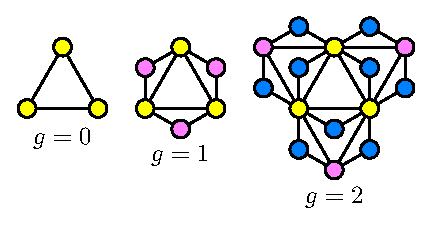
\includegraphics[width=0.75\linewidth]{Pseudofractal.eps}
		\caption{ Illustration of the first several iterations of the pseudofractal scale-free web. }
		\label{psfw1}
	\end{center}
\end{figure}
%%%%%%%%%%%%%%%%%%%%%%%%%%%%%%%%%%%%%%%%%%%%%%%%%%%%%%%%%%


The Koch network is also built in an iterative way. Let $\mathcal{M}_{g}$ ($g \geq 0$) denote the Koch network after $g$ iterations. Initially ($g=0$), $\mathcal{M}_{0}$ is a triangle with three
vertices and three edges. For $g\geq 1$, $\mathcal{M}_{g}$ is obtained from $\mathcal{M}_{g-1}$ by
performing the following operations. For each of the three vertices in
every existing triangle in $\mathcal{M}_{g-1}$, two new vertices are created, both of which and their
``mother'' vertices are connected to one another forming a new triangle. Figure~\ref{network} illustrates the growth process of the Koch network.  In network $\mathcal{M}_{g}$, the number of vertices is $2\times 4^{g}+1$, and the number of
edges is $3\times 4^{g}$.  In~\cite{XiLiZh15}, the Kemeny constant $K(\mathcal{M}_g)$ for $\mathcal{M}_g$ was obtained to be
\begin{equation}\label{Kg02}
	K(\mathcal{M}_g)=(1+2g)\times 4^g+\frac{1}{3}\,. %\notag
\end{equation}

%%%%%%%%%%%%%%%%%%%%%%%%%%%%%%%%%%%%%%%%%%%%%%%%%%%%%%%%%
% Figure 2
%%%%%%%%%%%%%%%%%%%%%%%%%%%%%%%%%%%%%%%%%%%%%%%%%%%%%
\begin{figure}
	\centering
	\includegraphics[width=0.85\linewidth,trim=0 0 0 0]{Koch.eps}
	%\includegraphics[width=0.5\textwidth]{Labelling.eps}
	\caption{Construction process for the Koch network.}
	\label{network}
\end{figure}
%%%%%%%%%%%%%%%%%%%%%%%%%%%%%%%%%%%%%%%%%%%%%%%%%%%%%

We use our  algorithm $\text{Approx}\mathcal{HK}$ to compute the Kemeny constant on  pseudofractal scale-free web $\mathcal{F}_{12}$ and the Koch network $\mathcal{M}_{10}$. The numerical results are reported in  Table~\ref{tab:Kemeny}, which shows that the approximation algorithm $\text{Approx}\mathcal{HK}$ works effectively for both networks. This again demonstrates the advantage of our proposed algorithm for large networks.


%%%%%%%%%%%%%%%%%%%%%%%%%%%%%%%%%%%%%%%%%%%%%%%
\begin{table*}[htbp]
	%\tabcolsep=5pt
	\centering
	\normalsize
	%\fontsize{6.51}{8.0}\selectfont
	\begin{threeparttable}
		\caption{Exact Kemeny constant $K$,   their approximation $\tilde{K}$,  relative error $\rho=(K-\tilde{K})/K$, and running time (seconds, $s$) for $\tilde{K}$ on networks $\mathcal{F}_{12}$ and $\mathcal{M}_{10}$.  $K$ is obtained via~\eqref{Kg01} and~\eqref{Kg02}, while $\tilde{K}$ is obtained through algorithm $\text{Approx}\mathcal{HK}$ with $\epsilon=0.1$.}
		\label{tab:Kemeny}
		\begin{tabular}{ccccccc}
			\toprule
			Network            & Vertices  & Edges     & $K$        & $\tilde{K}$ & Error $\rho$ & Time\cr
			\midrule
			\specialrule{0em}{3pt}{3pt}
			$\mathcal{F}_{12}$ & 797,163   & 1,594,323 & 1,321,776  & 1,321,956   & 0.00014      & 207\cr
			\specialrule{0em}{3pt}{3pt}
			$\mathcal{M}_{10}$ & 2,097,153 & 3,145,728 & 22,020,096 & 22,018,022  & 0.000094     & 1917\cr
			\specialrule{0em}{3pt}{3pt}
			%ZGL	           & 1,594,324  & 1,594,323  & 14,348,907 & 14,341,659\cr
			%\specialrule{0em}{3pt}{3pt}
			%ABZ			& 1,572,862  & 1,572,861 & 52,953,206 & 53,010,203\cr
			%\specialrule{0em}{3pt}{3pt}
			%DA			& 2,125,764  & 3,188,646 & 975,712,194 & 959,864,749\cr
			\bottomrule
		\end{tabular}
	\end{threeparttable}
\end{table*}
%%%%%%%%%%%%%%%%%%%%%%%%%%%%%%%%%%%%%%%%%%%%%%%

%\begin{table}[htbp]
%	\tabcolsep=5pt
%	\centering
%	\fontsize{8}{8}\selectfont
%	\begin{threeparttable}
%		\caption{Exact Kemeny constant $K$ and its approximation $\hat{K}$ with various $\epsilon$.}
%		\label{tab:accuracy}
%		\begin{tabular}{cccccc}
%			\toprule
%			\multirow{2}{*}{Network}&
%			\multirow{2}{*}{$n$}&
%			\multirow{2}{*}{$m$}&
%			\multirow{2}{*}{$K$}&
%			\multicolumn{2}{c}{$\hat{K}$ with various $\epsilon$}\cr
%			\cmidrule{5-6}
%			& & & & $0.2$ & $0.1$\cr
%			\midrule
%			\specialrule{0em}{3pt}{3pt}
%			Koch             & 2,097,153  & 3,145,728  & 22,020,096 & 21,944,591 & 22,018,022\cr
%			\specialrule{0em}{3pt}{3pt}
%			ZLG              & 797,163   & 1,594,323  & 1,321,776 & 1,322,092 & 1,321,956\cr
%			\specialrule{0em}{3pt}{3pt}
%			ZGL	           & 1,594,324  & 1,594,323  & 14,348,907 & 14,307,630 & 14,341,659\cr
%			\specialrule{0em}{3pt}{3pt}
%			ABZ			& 1,572,862  & 1,572,861 & 52,953,206 & 53,318,986 & 53,010,203\cr
%			\specialrule{0em}{3pt}{3pt}
%			DA			& 2,125,764  & 3,188,646 & 975,712,194 & 1,004,722,850 & 959,864,749\cr
%			\bottomrule
%		\end{tabular}
%	\end{threeparttable}
%\end{table}

%\begin{table*}[ht]
%	\centering
%	\fontsize{8}{8}\selectfont
%	\begin{threeparttable}
%		\begin{tabular}{ccccccccccccccc}
%			\Xhline{2\arrayrulewidth}
%			\multirow{2}{*}{Network}&
%			\multirow{2}{*}{$\mathtt{Exact\mathcal{H}}$}&
%			\multicolumn{6}{c}{$\mathtt{Exact\mathcal{H}}$ ($s$) with various $\epsilon$}&
%			\multirow{2}{*}{$\mathtt{Exact\mathcal{H}}$}&
%			\multicolumn{6}{c}{$\mathtt{Exact\mathcal{H}}$ ($s$) with various $\epsilon$}\cr
%			\cmidrule(lr){3-8}
%			\cmidrule(lr){10-15}
%			&   ($s$) & $0.3$ & $0.25$ & $0.2$ & $0.15$ & $0.1$ & $0.05$ & ($s$) & $0.3$ & $0.25$ & $0.2$ & $0.15$ & $0.1$ & $0.05$\cr
%			\midrule
%			Jazz musicians             & 0.0011  & 0.0205  & 0.0263 & 0.0434 & 0.0717 & 0.1441 & -- & 0.0010  & 0.0197  & 0.0278 & 0.0414 & 0.0686 & 0.1489& 0.5714 \cr
%			Chicago              & 0.0338  & 0.0075  & 0.0092 & 0.0138 & 0.0238 & 0.0503 & -- & 0.0323  & 0.0076  & 0.0090 & 0.0137 & 0.0237 & 0.0504 & 0.1936\cr
%			Hamster full	     &0.3859  & 0.2262 & 0.2651 & 0.4052 & 0.7034 & 1.5913 & -- &0.3720  & 0.2009 & 0.3089 & 0.4358 & 0.7499 & 1.5766 & 6.2718\cr
%			Facebook (NIPS)	    &2.8894  & 0.9651 & 1.3385 & 1.9728 & 3.4080 & 7.5011 & --  &2.7580  & 1.0608 & 1.2899 & 2.1198 & 3.6758 & 7.5303 & 30.819 \cr
%			CA-GrQc             &3.1277  & 0.3065 & 0.3838  & 0.5901 & 1.0391 & 2.3361 & -- &2.9978  & 0.3368 & 0.3867  & 0.5711 & 1.1744 & 2.3367 & 9.4107\cr
%			Reactome            &8.8248  & 1.7534 & 2.4701  & 3.7091 & 6.0085 & 13.881 & -- &8.5989  & 1.8765 & 2.4432  & 3.7009 & 6.4243 & 13.454 & 56.133\cr
%			Route views         &11.350  & 0.2865 & 0.3511 & 0.5357 & 0.9806 & 1.9931 & -- &10.881  & 0.2618 & 0.3336 & 0.4860 & 0.9325 & 2.0380 & 7.7761\cr
%			Pretty Good Privacy & 47.796 & 0.7460 & 0.9072 & 1.4505 & 2.4947 & 5.9288 & -- & 46.792 & 0.7516 & 0.9175 & 1.5451 & 2.5512 & 5.9918 & 22.201\cr
%			CA-HepPh      		& 54.393 & 1.9375 & 2.4968 & 3.7927 & 7.0185 & 15.359 & -- & 53.974 & 1.9525 & 2.5085 & 3.5409 & 7.3778 & 14.640 & 58.654\cr
%			Astro-ph      		& 219.28 & 4.9590 & 4.7892 & 7.2232 & 13.329 & 29.616 & -- & 216.69 & 4.8033 & 5.1184 & 7.7884 & 14.524 & 28.894 & 129.11\cr
%			CAIDA               & 706.31 & 1.7242 & 1.7775 & 2.7819 & 4.7319 & 10.514 & -- & 700.85 & 1.7034 & 1.7467 & 2.7231 & 5.1186 & 10.402 & 42.167\cr
%			Brightkite          & 4589.0 & 8.5956 & 9.0904 & 13.818& 24.500 & 49.398 & -- & 4415.5 & 9.2414 & 8.2688 & 12.619& 21.880 & 51.511 & 212.84\cr
%			Livemocha*           &-- & 57.331 & 79.598 & 125.70 & 210.05 & 464.37 & -- &-- & 62.166 & 79.850 & 130.54 & 207.83 & 482.28 & 1842.5\cr
%			WordNet*             &-- & 23.033 & 31.516 & 48.151 & 96.365 & 188.43 & -- &-- & -- & -- & -- & -- & -- & --\cr
%			Gowalla*             &-- & 36.762 & 52.336 & 73.403 & 130.52 & 312.03 & -- &-- & 36.665 & 49.448 & 79.380 & 131.35 & 296.82 & 1241.1\cr
%			com-DBLP*              &-- & 57.132 & 90.414 & 143.40 & 248.81 & 511.22 & -- &-- & 60.977 & 89.687 & 126.97 & 240.35 & 522.27 & 2090.5\cr
%			Amazon*             &-- & 86.324 & 116.69 & 170.94 & 303.04 & 709.06 & -- &-- & 80.013 & 111.09 & 177.53 & 279.91 & 694.34 & 2604.5\cr
%			Pennsylvania*        &-- & 290.43 & 433.10 & 647.10 & 1103.6 & 2701.4 & -- & -- & 297.76 & 389.31 & 642.57 & 1160.7 & 2582.8 & --\cr
%			roadNet-TX*        &-- & 372.41 & 601.70 & 926.15 & 1555.3 & 3301.5 & -- &-- & -- & -- & -- & -- & -- & --\cr
%			\Xhline{2\arrayrulewidth}
%		\end{tabular}
%		\caption{The running time (seconds, $s$) of $\mathtt{Exact\mathcal{H}}$ and $\mathtt{Exact\mathcal{H}}$ with various $\epsilon$ on several real-world networks}
%		\label{tab:runtime_comparison}
%	\end{threeparttable}
%\end{table*}

%\begin{table*}[bp]
%	\centering
%	\tabcolsep=4.3pt
%	\small
%	%	\fontsize{8}{8}\selectfont
%	\begin{threeparttable}
%		\begin{tabularx}{\linewidth}{ccccccccccccccc}
%			\Xhline{2\arrayrulewidth}
%			\multirow{2}{*}{Network}&
%			\multirow{2}{*}{$\mathtt{Exact\mathcal{H}}$}&
%			\multicolumn{6}{c}{$\mathtt{Exact\mathcal{H}}$ ($s$) with various $\epsilon$}&
%			\multirow{2}{*}{$\mathtt{Exact\bar{C}}$}&
%			\multicolumn{6}{c}{$\mathtt{Appx\bar{C}}$ ($s$) with various $\epsilon$}\cr
%			\cmidrule(lr){3-8}
%			\cmidrule{10-15}
%			&   ($s$) & $0.3$ & $0.25$ & $0.2$ & $0.15$ & $0.1$ & $0.05$ & ($s$) & $0.3$ & $0.25$ & $0.2$ & $0.15$ & $0.1$ & $0.05$\cr
%			\midrule
%			Jazz musicians             & 0.001  & 0.020  & 0.026 & 0.043 & 0.071 & 0.144 & 0.613 & 0.001  & 0.019  & 0.027 & 0.041 & 0.068 & 0.148& 0.571 \cr
%			Chicago              & 0.033  & 0.007  & 0.009 & 0.013 & 0.023 & 0.050 & 0.204 & 0.03  & 0.007  & 0.009 & 0.013 & 0.023 & 0.05 & 0.193\cr
%			Hamster full	     &0.385  & 0.226 & 0.265 & 0.405 & 0.703 & 1.591 & 6.317 &0.372  & 0.200 & 0.308 & 0.435 & 0.749& 1.576 & 6.271\cr
%			Facebook (NIPS)	    &2.889  & 0.965 & 1.338 & 1.972 & 3.408 & 7.501 & 30.92  &2.758  & 1.060 & 1.289 & 2.119 & 3.675 & 7.530 & 30.81 \cr
%			CA-GrQc             &3.127  & 0.306 & 0.383  & 0.590 & 1.039 & 2.336 & 9.345 &2.997  & 0.336 & 0.386  & 0.571 & 1.174 & 2.336 & 9.410\cr
%			Reactome            &8.824  & 1.753 & 2.470  & 3.709 & 6.008 & 13.88 & 56.09 &8.598  & 1.876 & 2.443 & 3.700 & 6.424 & 13.45 & 56.13\cr
%			Route views         &11.35  & 0.286 & 0.351 & 0.535 & 0.980 & 1.993 & 7.907 &10.88  & 0.261 & 0.333 & 0.486 & 0.932 & 2.038 & 7.776\cr
%			Pretty Good Privacy & 47.79 & 0.746 & 0.907 & 1.450 & 2.494 & 5.928 & 21.17 & 46.79 & 0.751 & 0.917 & 1.545 & 2.551 & 5.991 & 22.20\cr
%			CA-HepPh      		& 54.39 & 1.937 & 2.496 & 3.792 & 7.018 & 15.35 & 57.16 & 53.97 & 1.952 & 2.508 & 3.540 & 7.377 & 14.64 & 58.65\cr
%			Astro-ph      		& 219.2 & 4.959 & 4.789 & 7.223 & 13.32 & 29.61 & 112.9 & 216.6 & 4.803 & 5.118 & 7.788 & 14.52 & 28.89 & 129.1\cr
%			CAIDA               & 706.3 & 1.724 & 1.777 & 2.781 & 4.731 & 10.51 & 42.90 & 700.8 & 1.703 & 1.746 & 2.723 & 5.118 & 10.40 & 42.16\cr
%			Brightkite          & 4589 & 8.595 & 9.090 & 13.81& 24.50 & 49.39 & 220.7 & 4415 & 9.241 & 8.268 & 12.61& 21.88 & 51.51 & 212.8\cr
%			Livemocha*           &-- & 57.33 & 79.59 & 125.7 & 210.0 & 464.3 & 1957 &-- & 62.16 & 79.85 & 130.5 & 207.8 & 482.2 & 1842\cr
%			WordNet*             &-- & 23.03 & 31.51 & 48.15 & 96.36 & 188.4 & 1112 &-- & 23.96 & 32.36 & 46.87 & 82.77 & 183.5 & 793.1\cr
%			Gowalla*             &-- & 36.76 & 52.33 & 73.40 & 130.5 & 312.0 & 1189 &-- & 36.66 & 49.44 & 79.38 & 131.3 & 296.8 & 1241\cr
%			com-DBLP*              &-- & 57.13 & 90.41 & 143.4 & 248.8 & 511.2 & 2250 &-- & 60.97 & 89.68 & 126.9 & 240.3 & 522.2 & 2090\cr
%			Amazon*             &-- & 86.32 & 116.6 & 170.9 & 303.0 & 709.0 & 2523 &-- & 80.01 & 111.0 & 177.5 & 279.9 & 694.3 & 2604\cr
%			Pennsylvania*        &-- & 290.4 & 433.1 & 647.1 & 1103. & 2701 & 13233 & -- & 301.7 & 443.2 & 672.8 & 1186 & 2823 & 10402\cr
%			roadNet-TX*        &-- & 372.4 & 601.7 & 926.1 & 1555 & 3301 & 17522 &-- & 405.3 & 548.1 & 883.4 & 1658 & 3478 & 14160\cr
%			\Xhline{2\arrayrulewidth}
%		\end{tabularx}
%		\caption{The running time (seconds, $s$) of $\mathtt{Exact\mathcal{H}}$, $\mathtt{Exact\bar{C}}$, $\mathtt{Exact\mathcal{H}}$ and $\mathtt{Appx\bar{C}}$ with various $\epsilon$ on several real-world networks}
%		\label{tab:runtime_comparison}
%	\end{threeparttable}
%\end{table*}



\section{Conclusions}

The hitting time of random walks arises  in many practical scenarios. However, the time cost of exactly computing hitting time is prohibitively expensive. In this paper, we studied a walk centrality and Kemeny constant of a graph, both of which are actually weighted average of hitting times and have found wide  applications. We established a link between the two quantities, and reformulated them in terms of quadratic forms of the pseudoinverse of graph Laplacian. Moreover, we provided a randomized approximation algorithm with probabilistic guarantee, which computes the walk centrality for all vertices and Kemeny constant in nearly linear time with respect to  the number of edges. Finally, we conducted extensive experiments on various real-world and model networks, which show that the proposed  algorithm is both efficient and accurate, especially for large-scale networks. %It is expected that our approximate method can be extended or modified to compute other quantities derived from hitting times~\cite{Lo93}.


%\section*{Acknowledgements}
\begin{acks}
	The work was supported by the National Natural Science
	Foundation of China under Grant 61872093, the National Key R \& D Program of China
	(No. 2018YFB1305104), Shanghai Municipal Science and Technology Major Project  (No.  2018SHZDZX01) and ZJLab. Zuobai Zhang was also supported by Fudan's Undergraduate Research Opportunities Program (FDUROP) under Grant No. 19914.
\end{acks}
%\newpage

\bibliographystyle{ACM-Reference-Format}
\balance
\bibliography{Hitting,Kemeny}

\end{document}
